\begin{figure*}
	\begin{subfigure}[t]{.49\linewidth}
		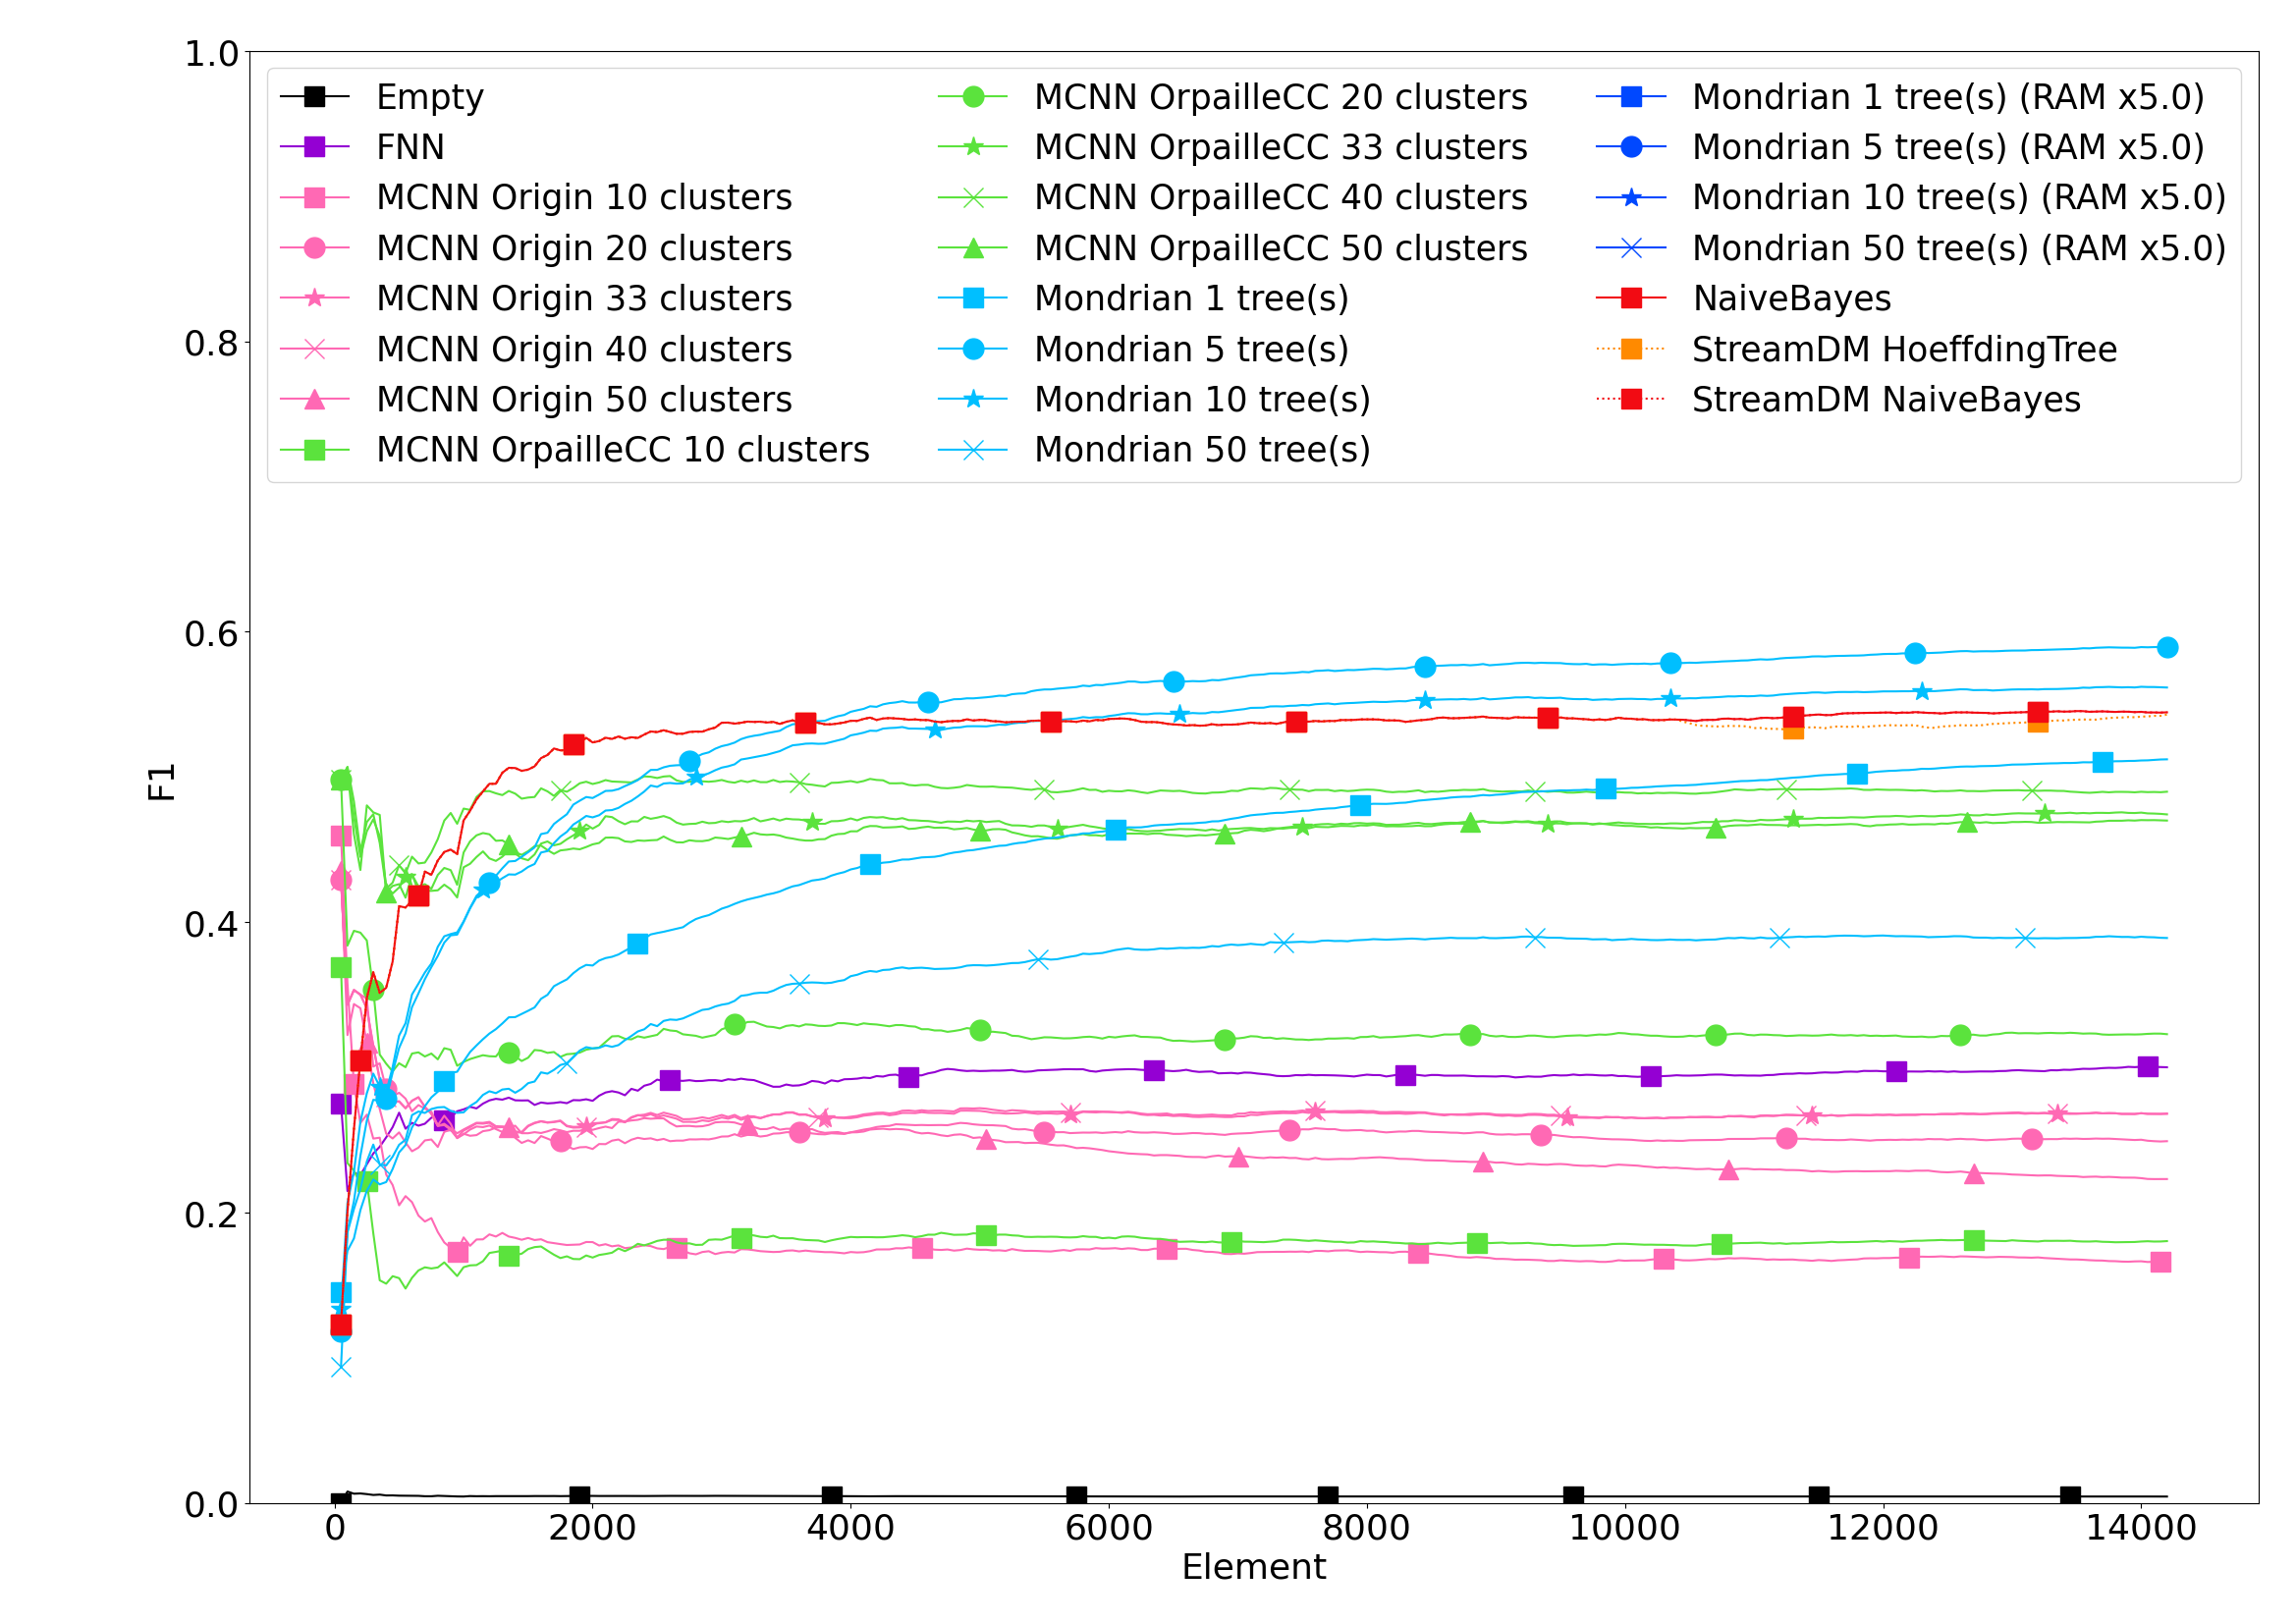
\includegraphics[width=\linewidth]{figures/results/banos_3_f1.png}
		\caption{\banosdataset}
		\label{fig:f1-banos}
	\end{subfigure}
	\hfill
	\begin{subfigure}[t]{.49\linewidth}
		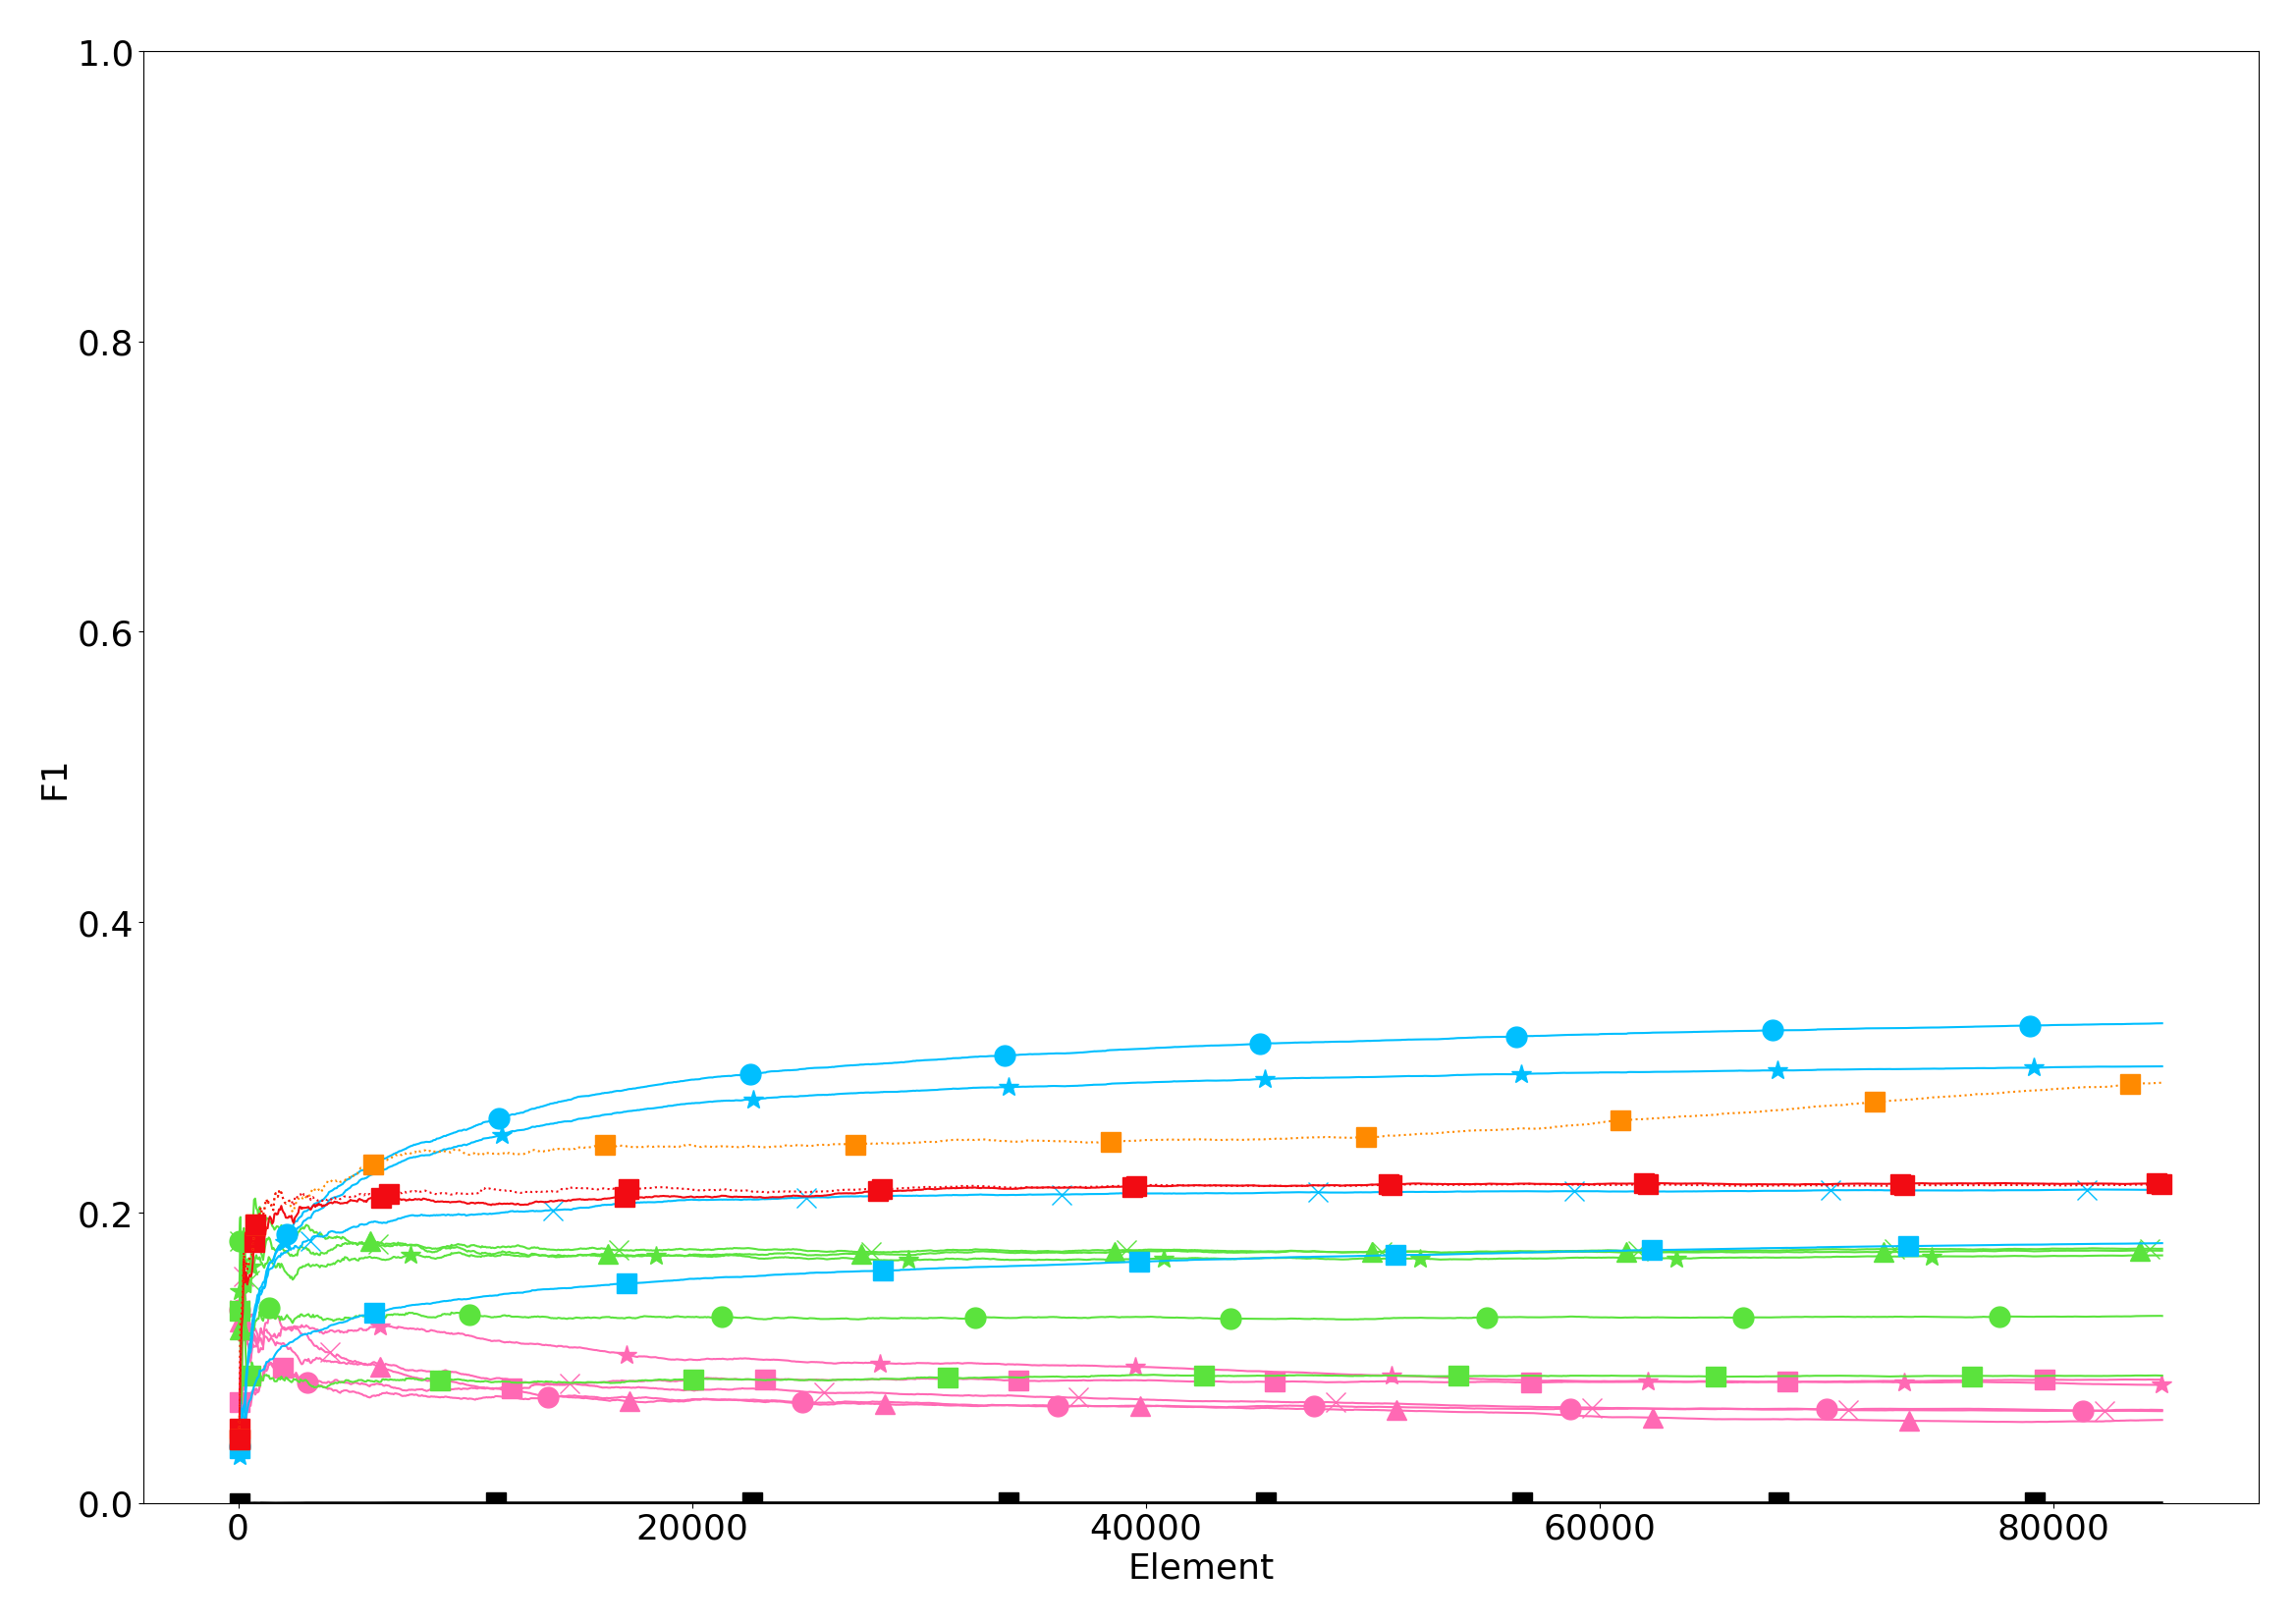
\includegraphics[width=\linewidth]{figures/results/recofit_3_f1.png}
		\caption{\recofitdataset}
		\label{fig:f1-recofit}
	\end{subfigure}\\
	\begin{subfigure}[t]{.49\linewidth}
		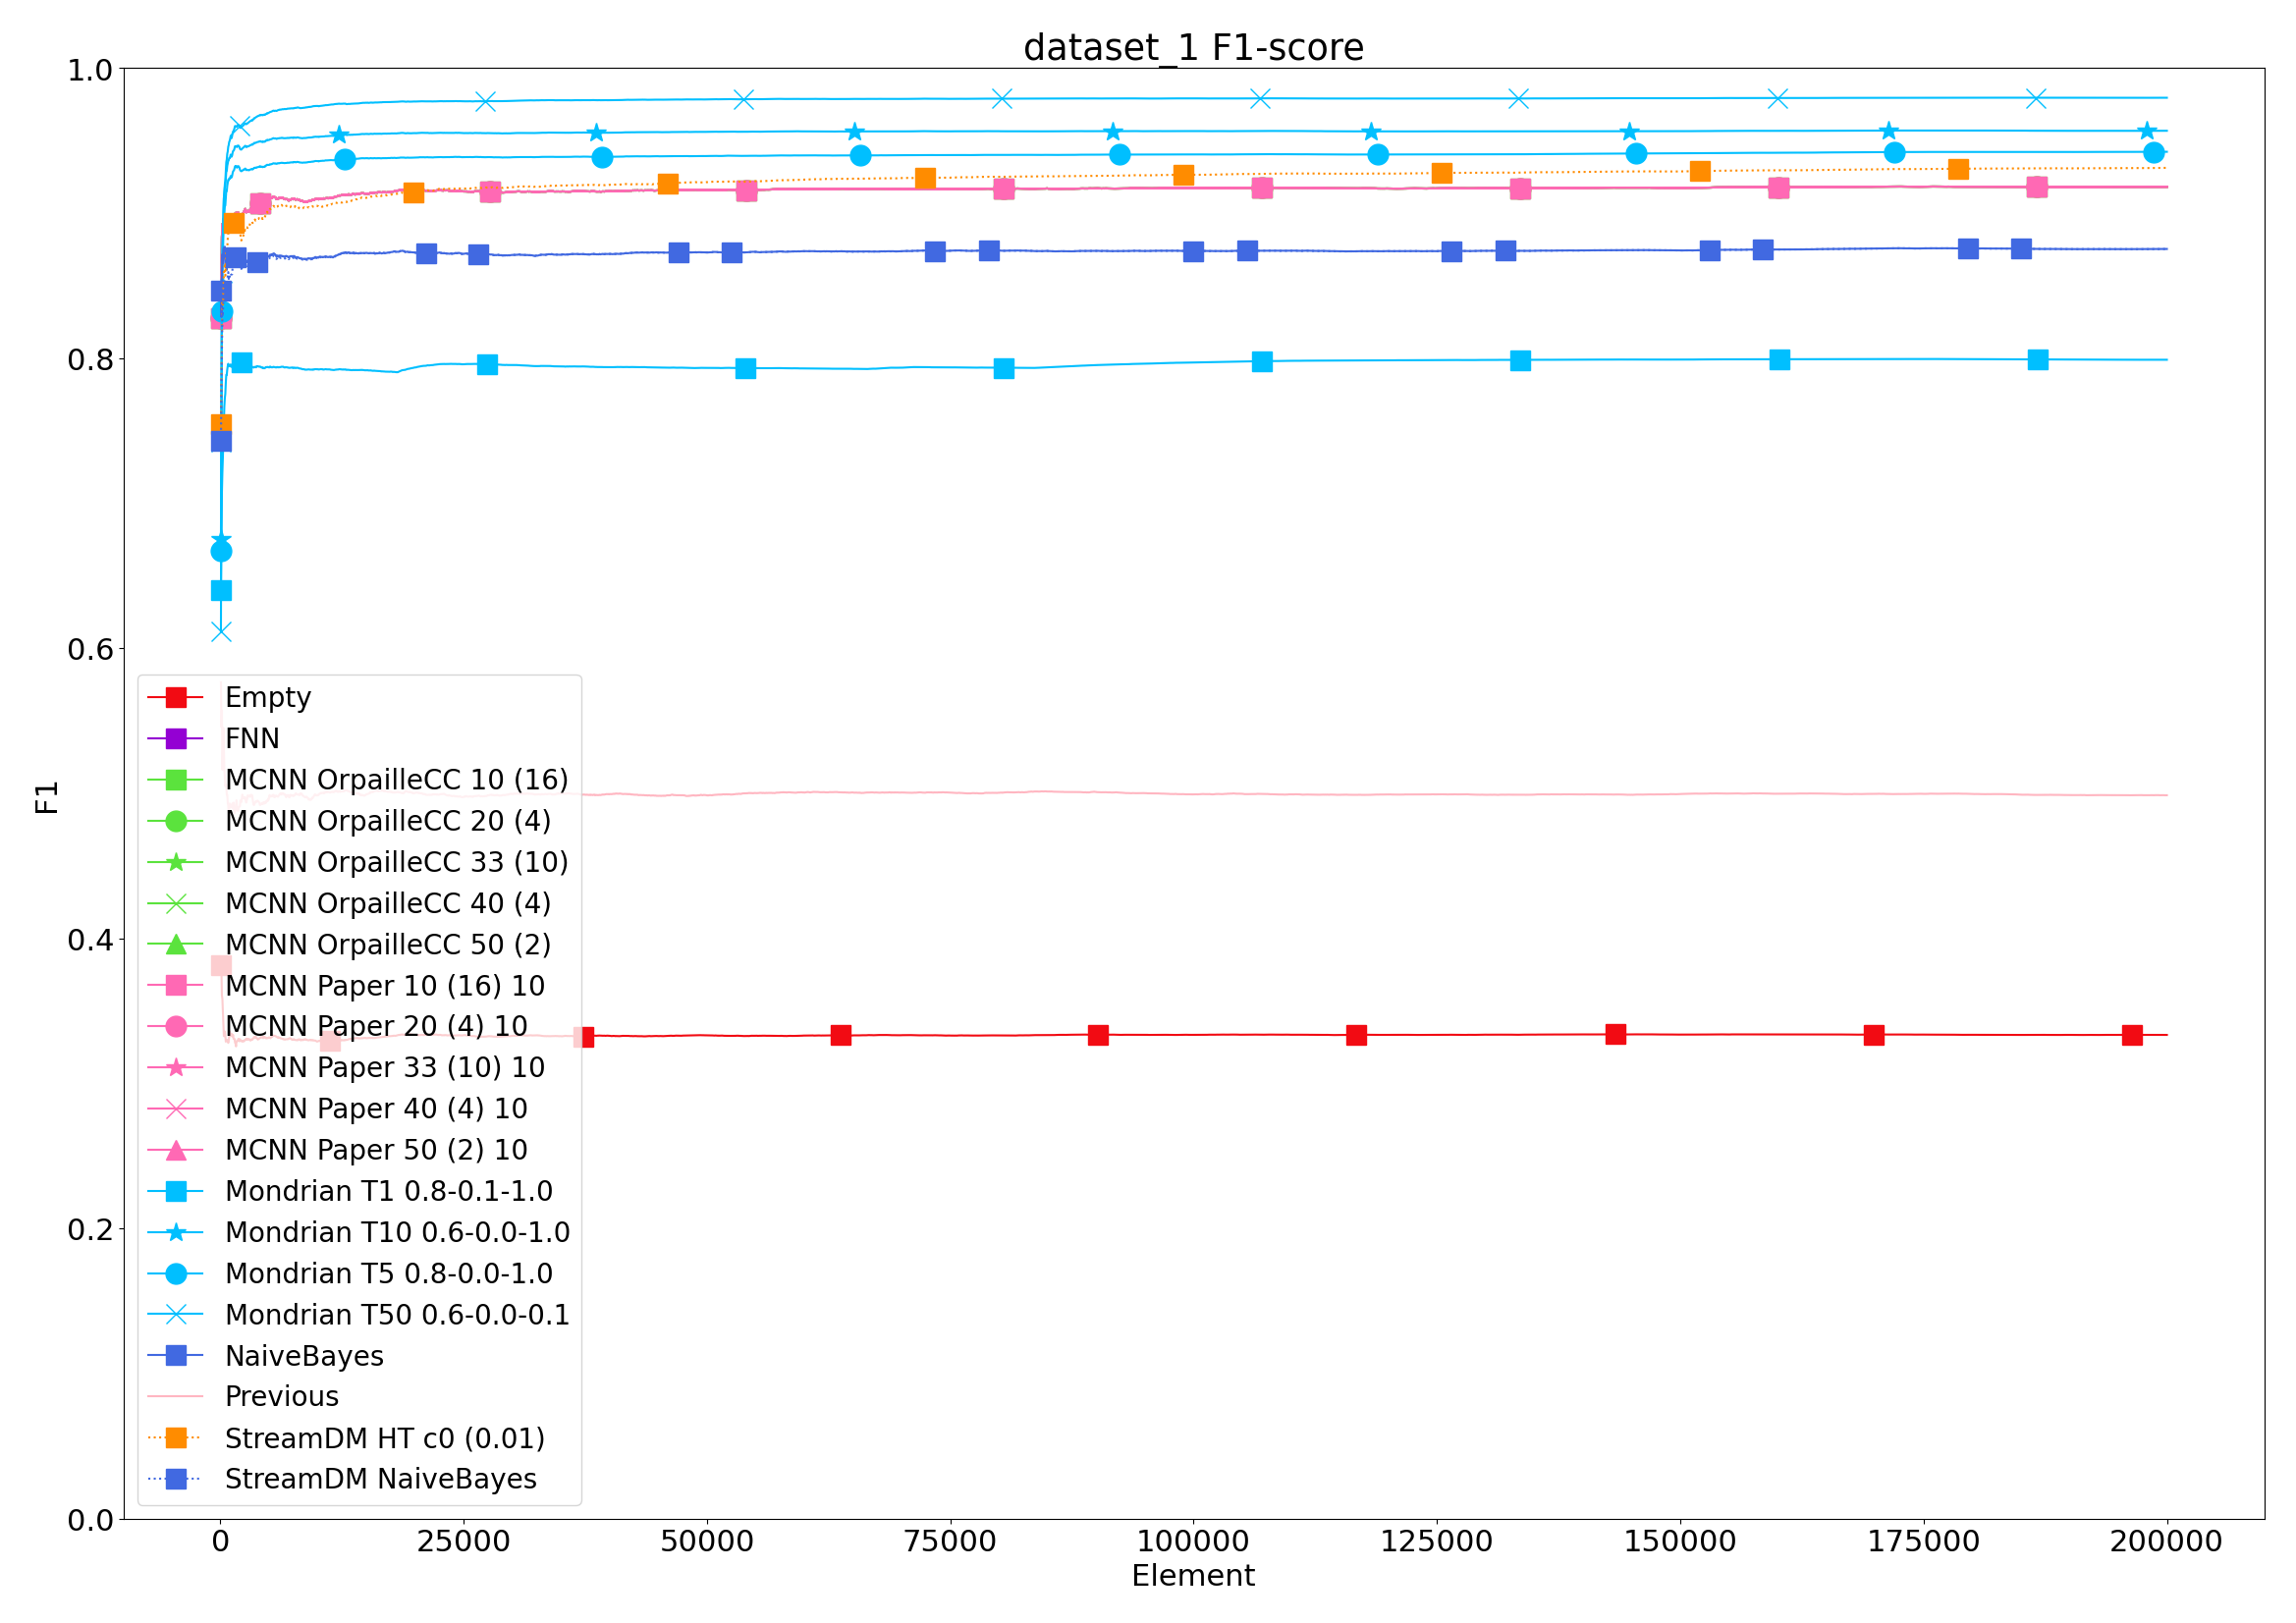
\includegraphics[width=\linewidth]{figures/results/dataset_1_f1.png}
		\caption{Hyperplane}
		\label{fig:f1-dataset_1}
	\end{subfigure}
	\hfill
	\begin{subfigure}[t]{.49\linewidth}
		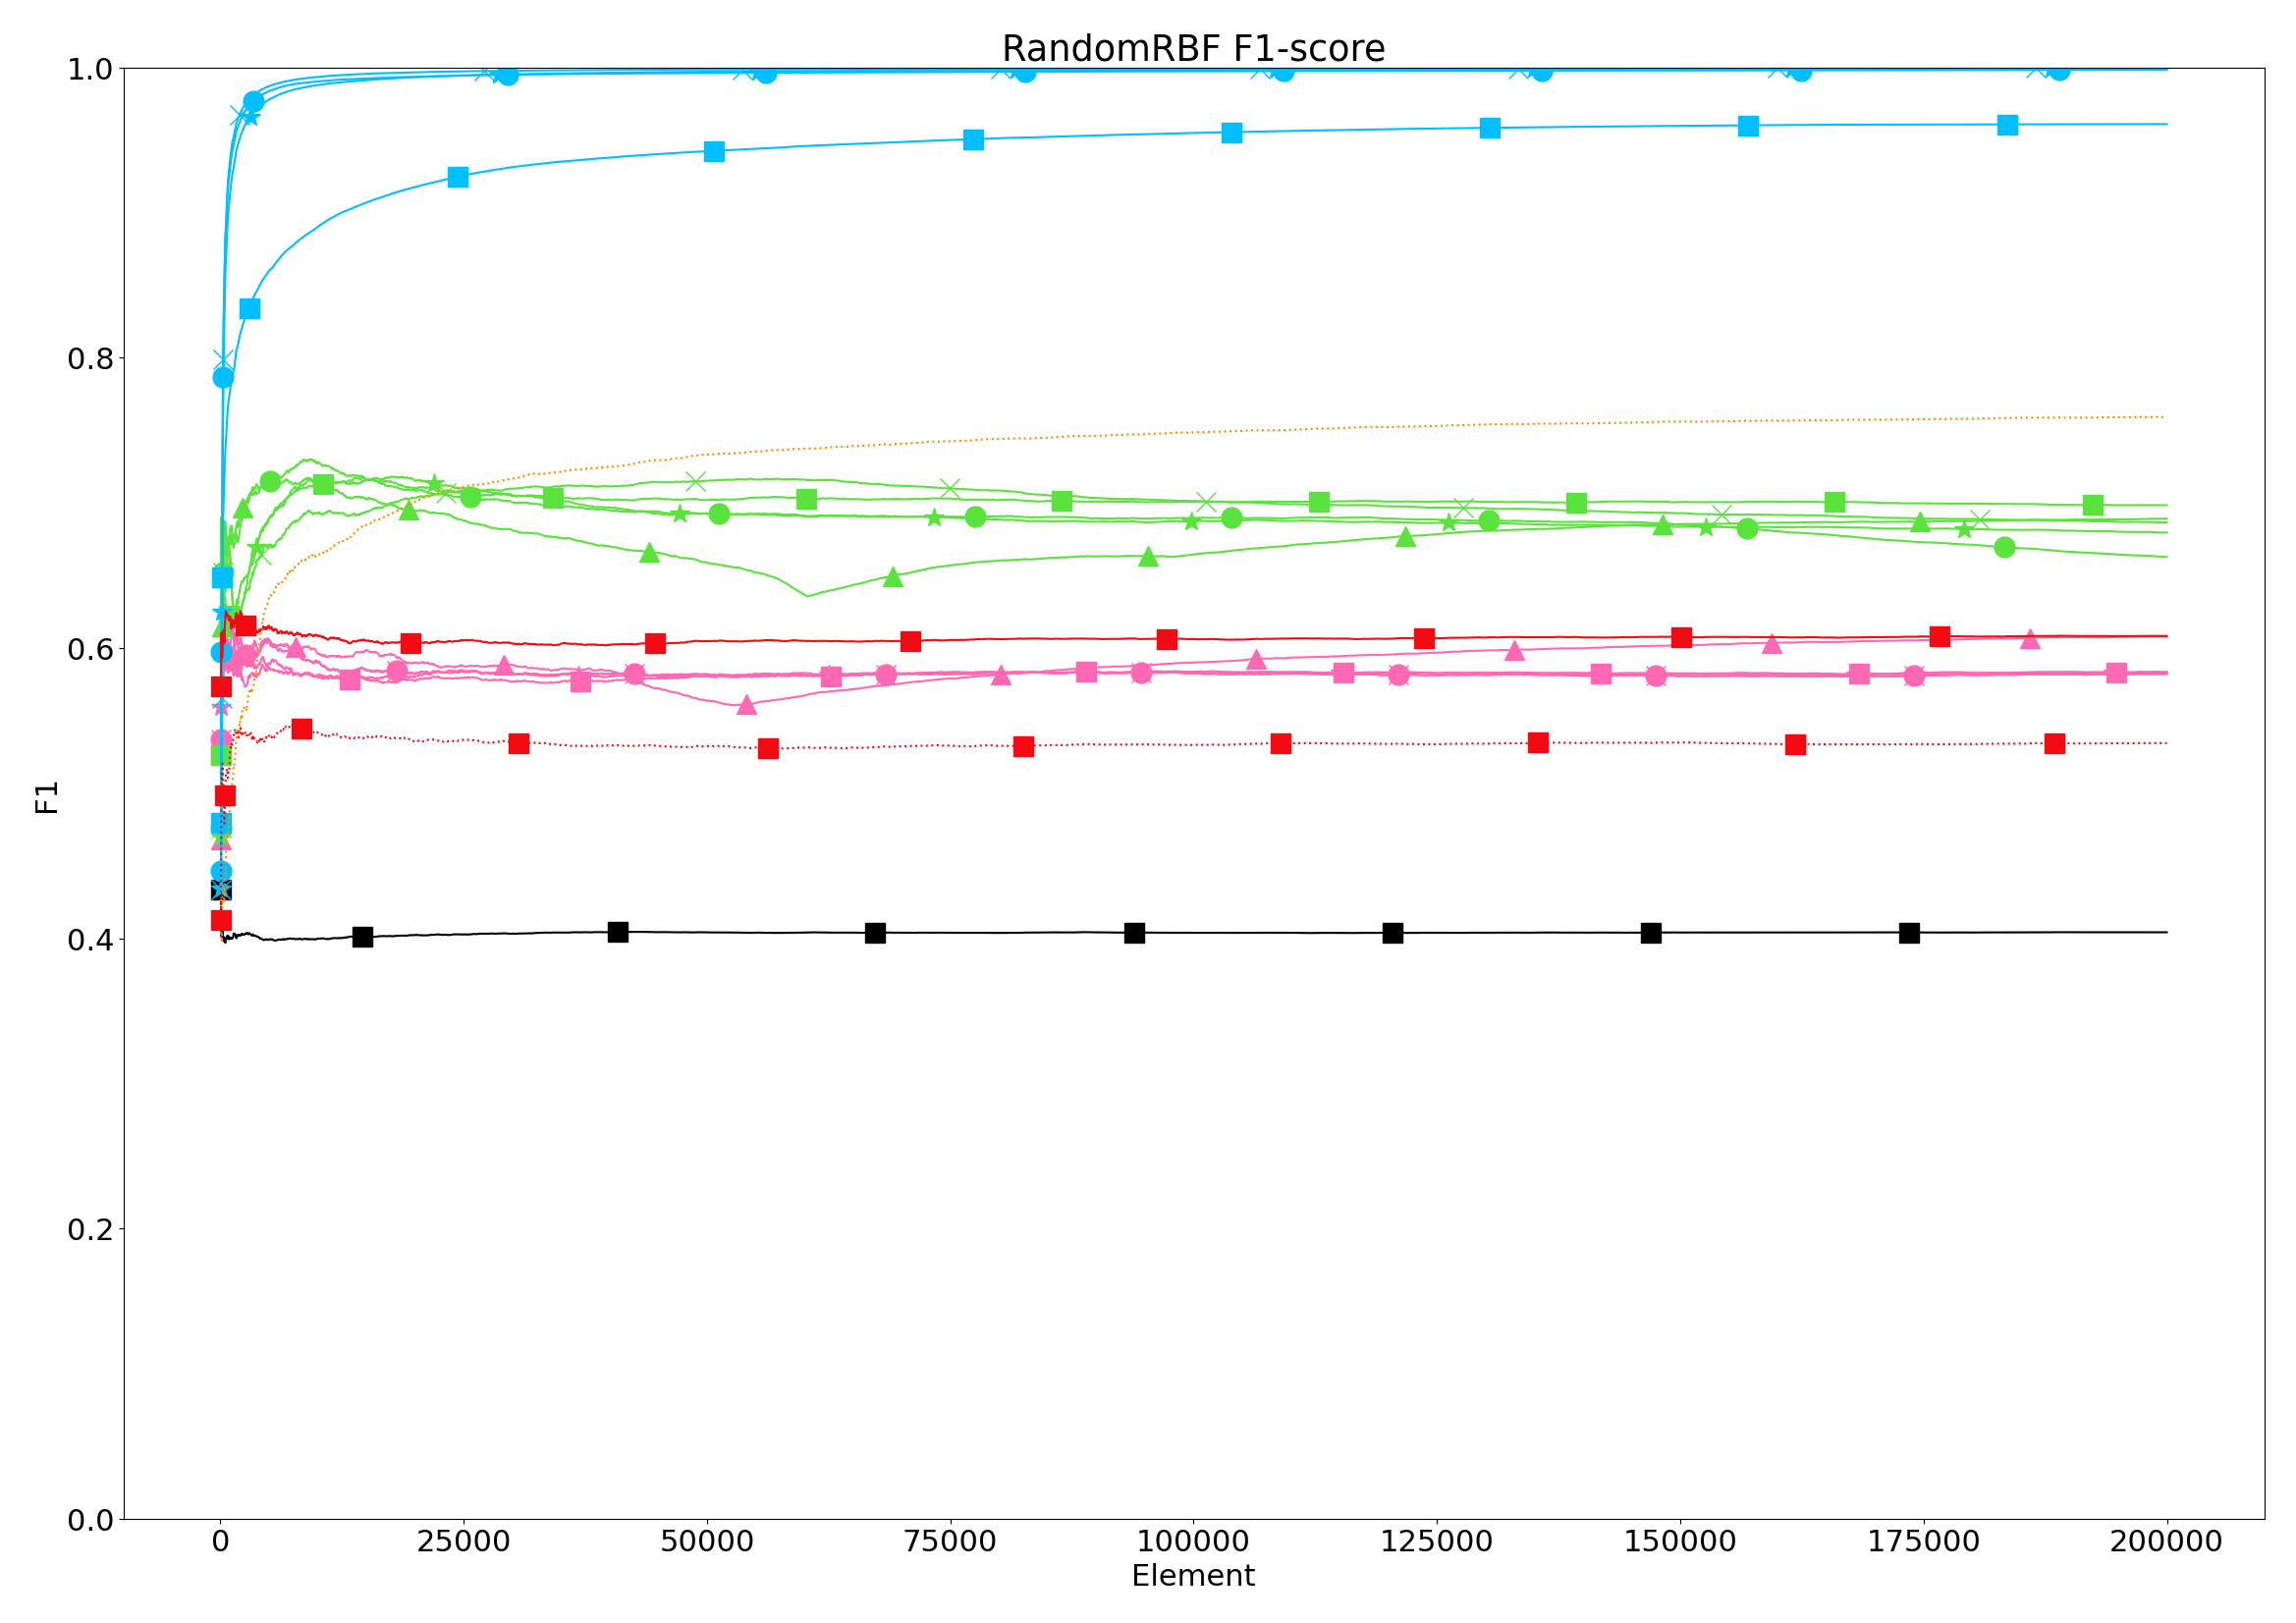
\includegraphics[width=\linewidth]{figures/results/dataset_2_f1.png}
		\caption{RandomRBF}
		\label{fig:f1-dataset_2}
	\end{subfigure}\\
	\begin{subfigure}[t]{.49\linewidth}
		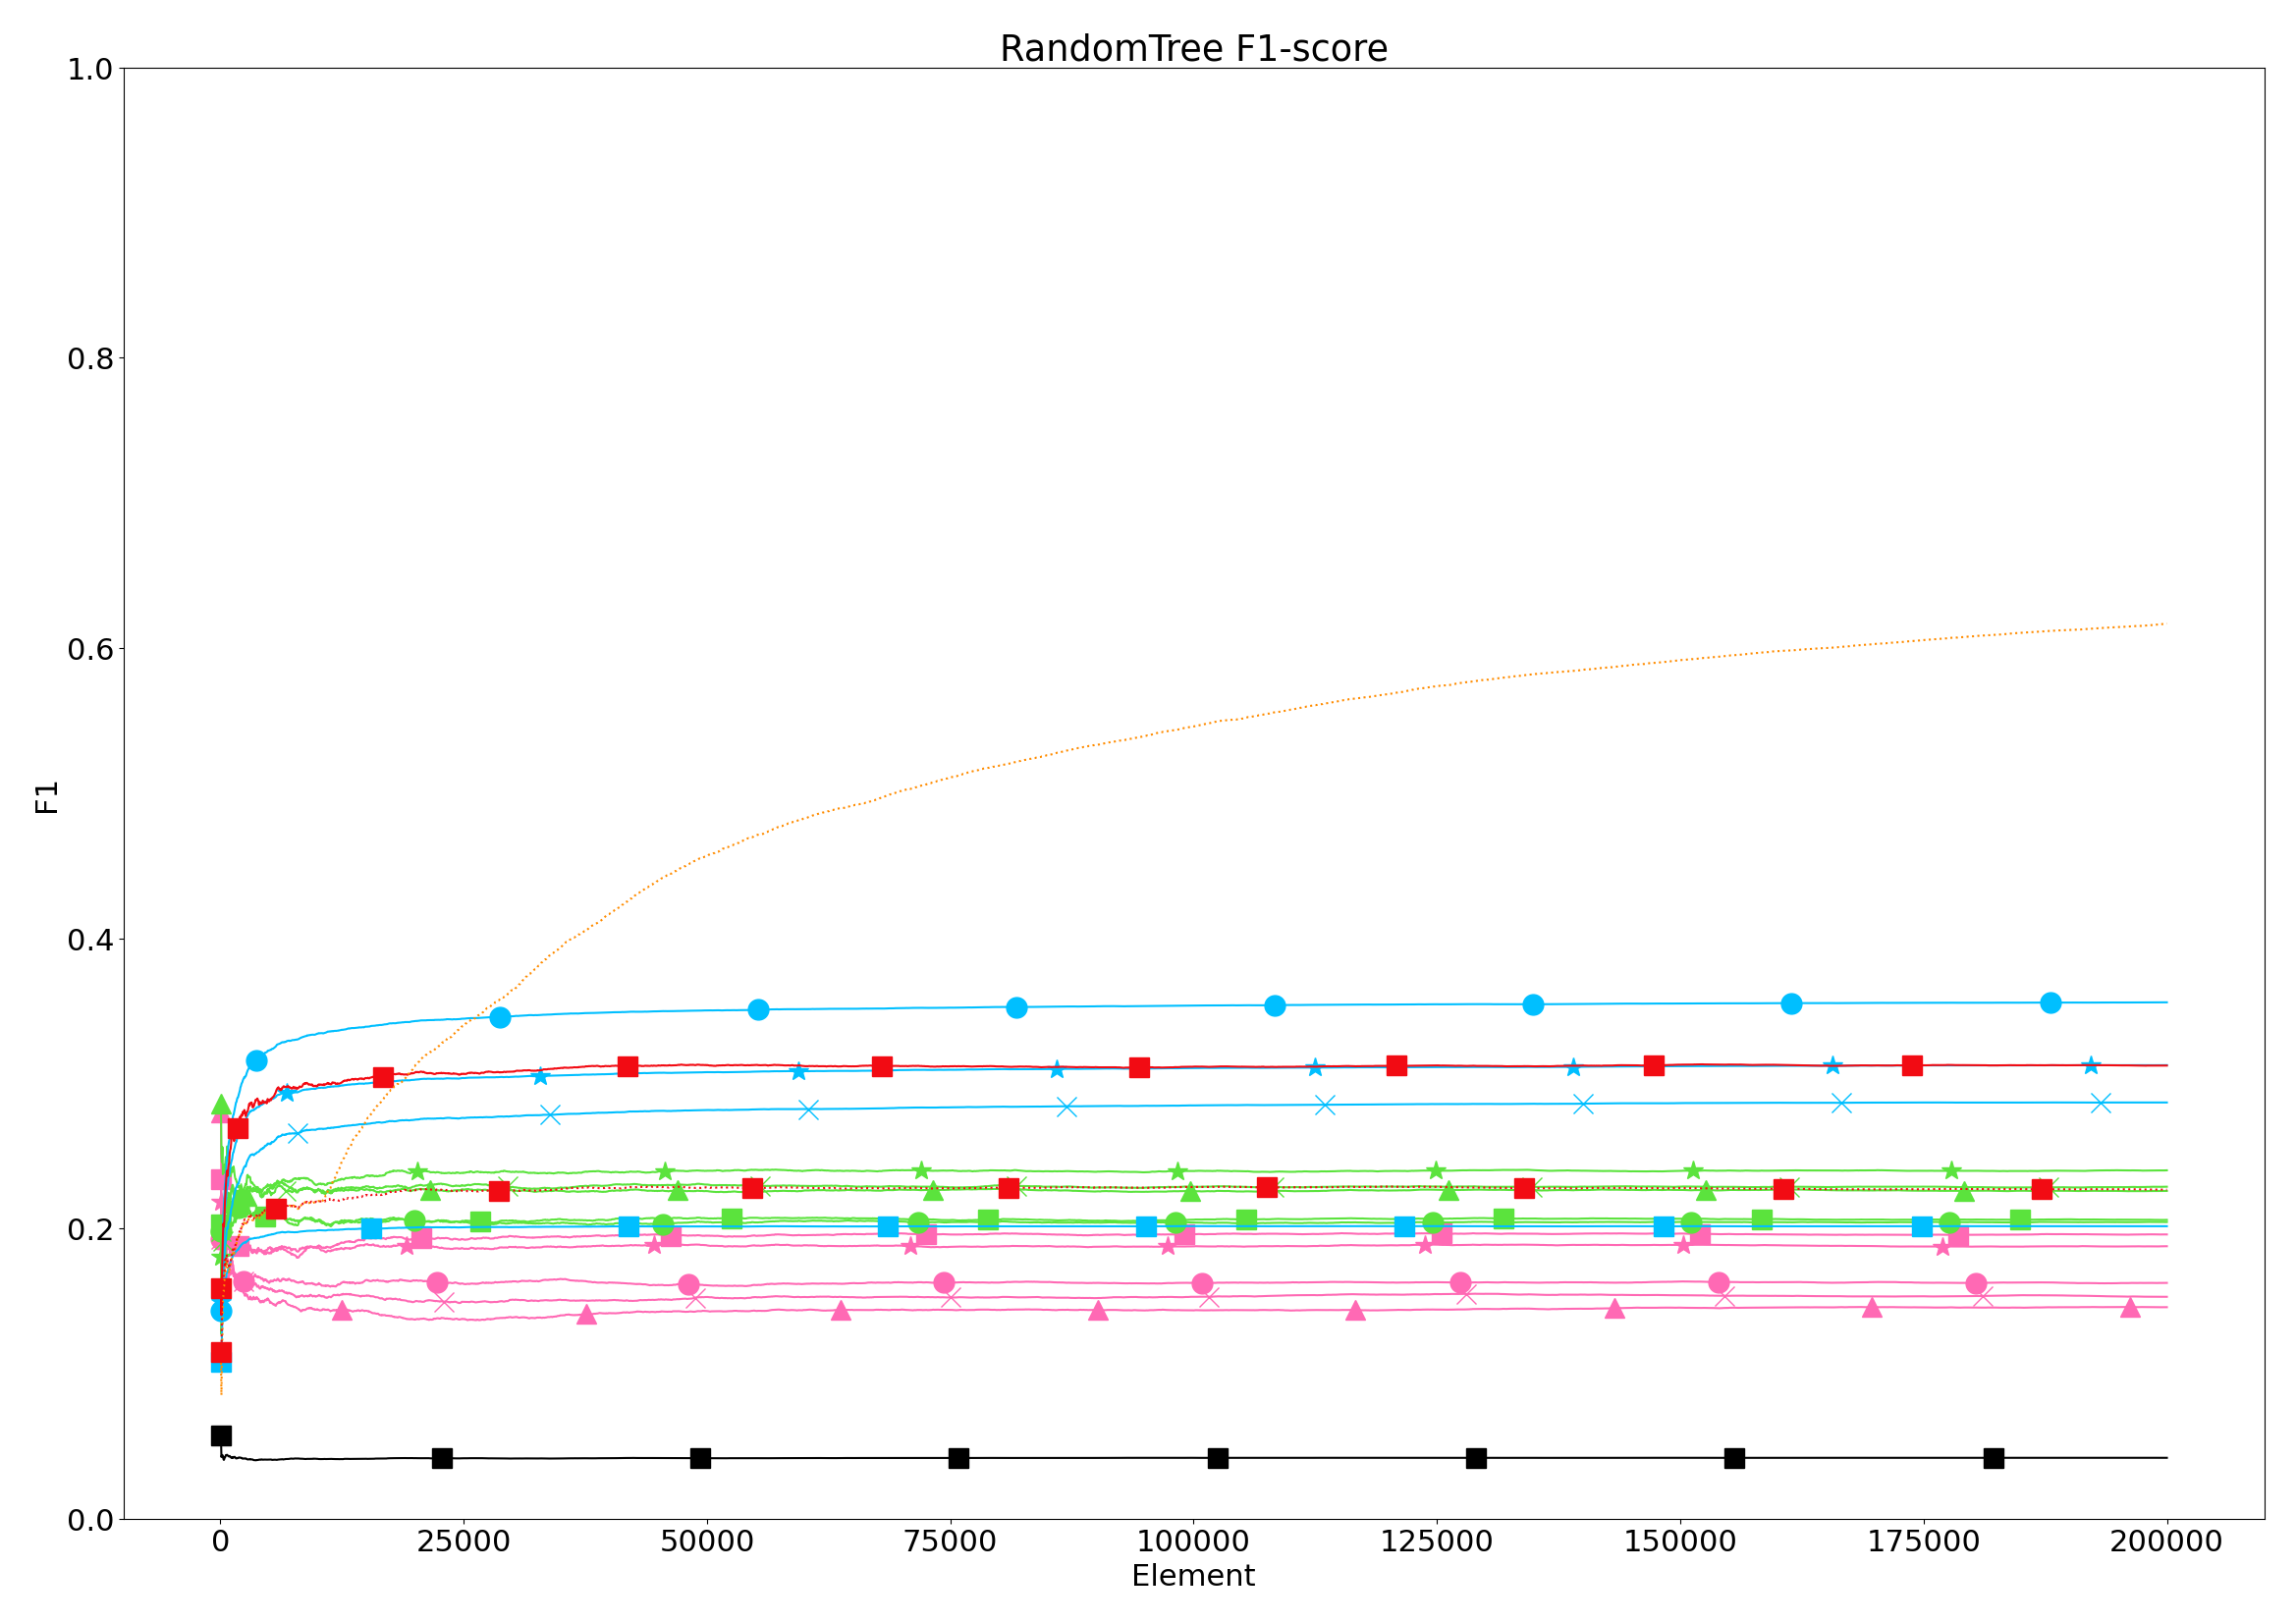
\includegraphics[width=\linewidth]{figures/results/dataset_3_f1.png}
		\caption{RandomTree}
		\label{fig:f1-dataset_3}
	\end{subfigure}
	\hfill
	\begin{subfigure}[t]{.49\linewidth}
		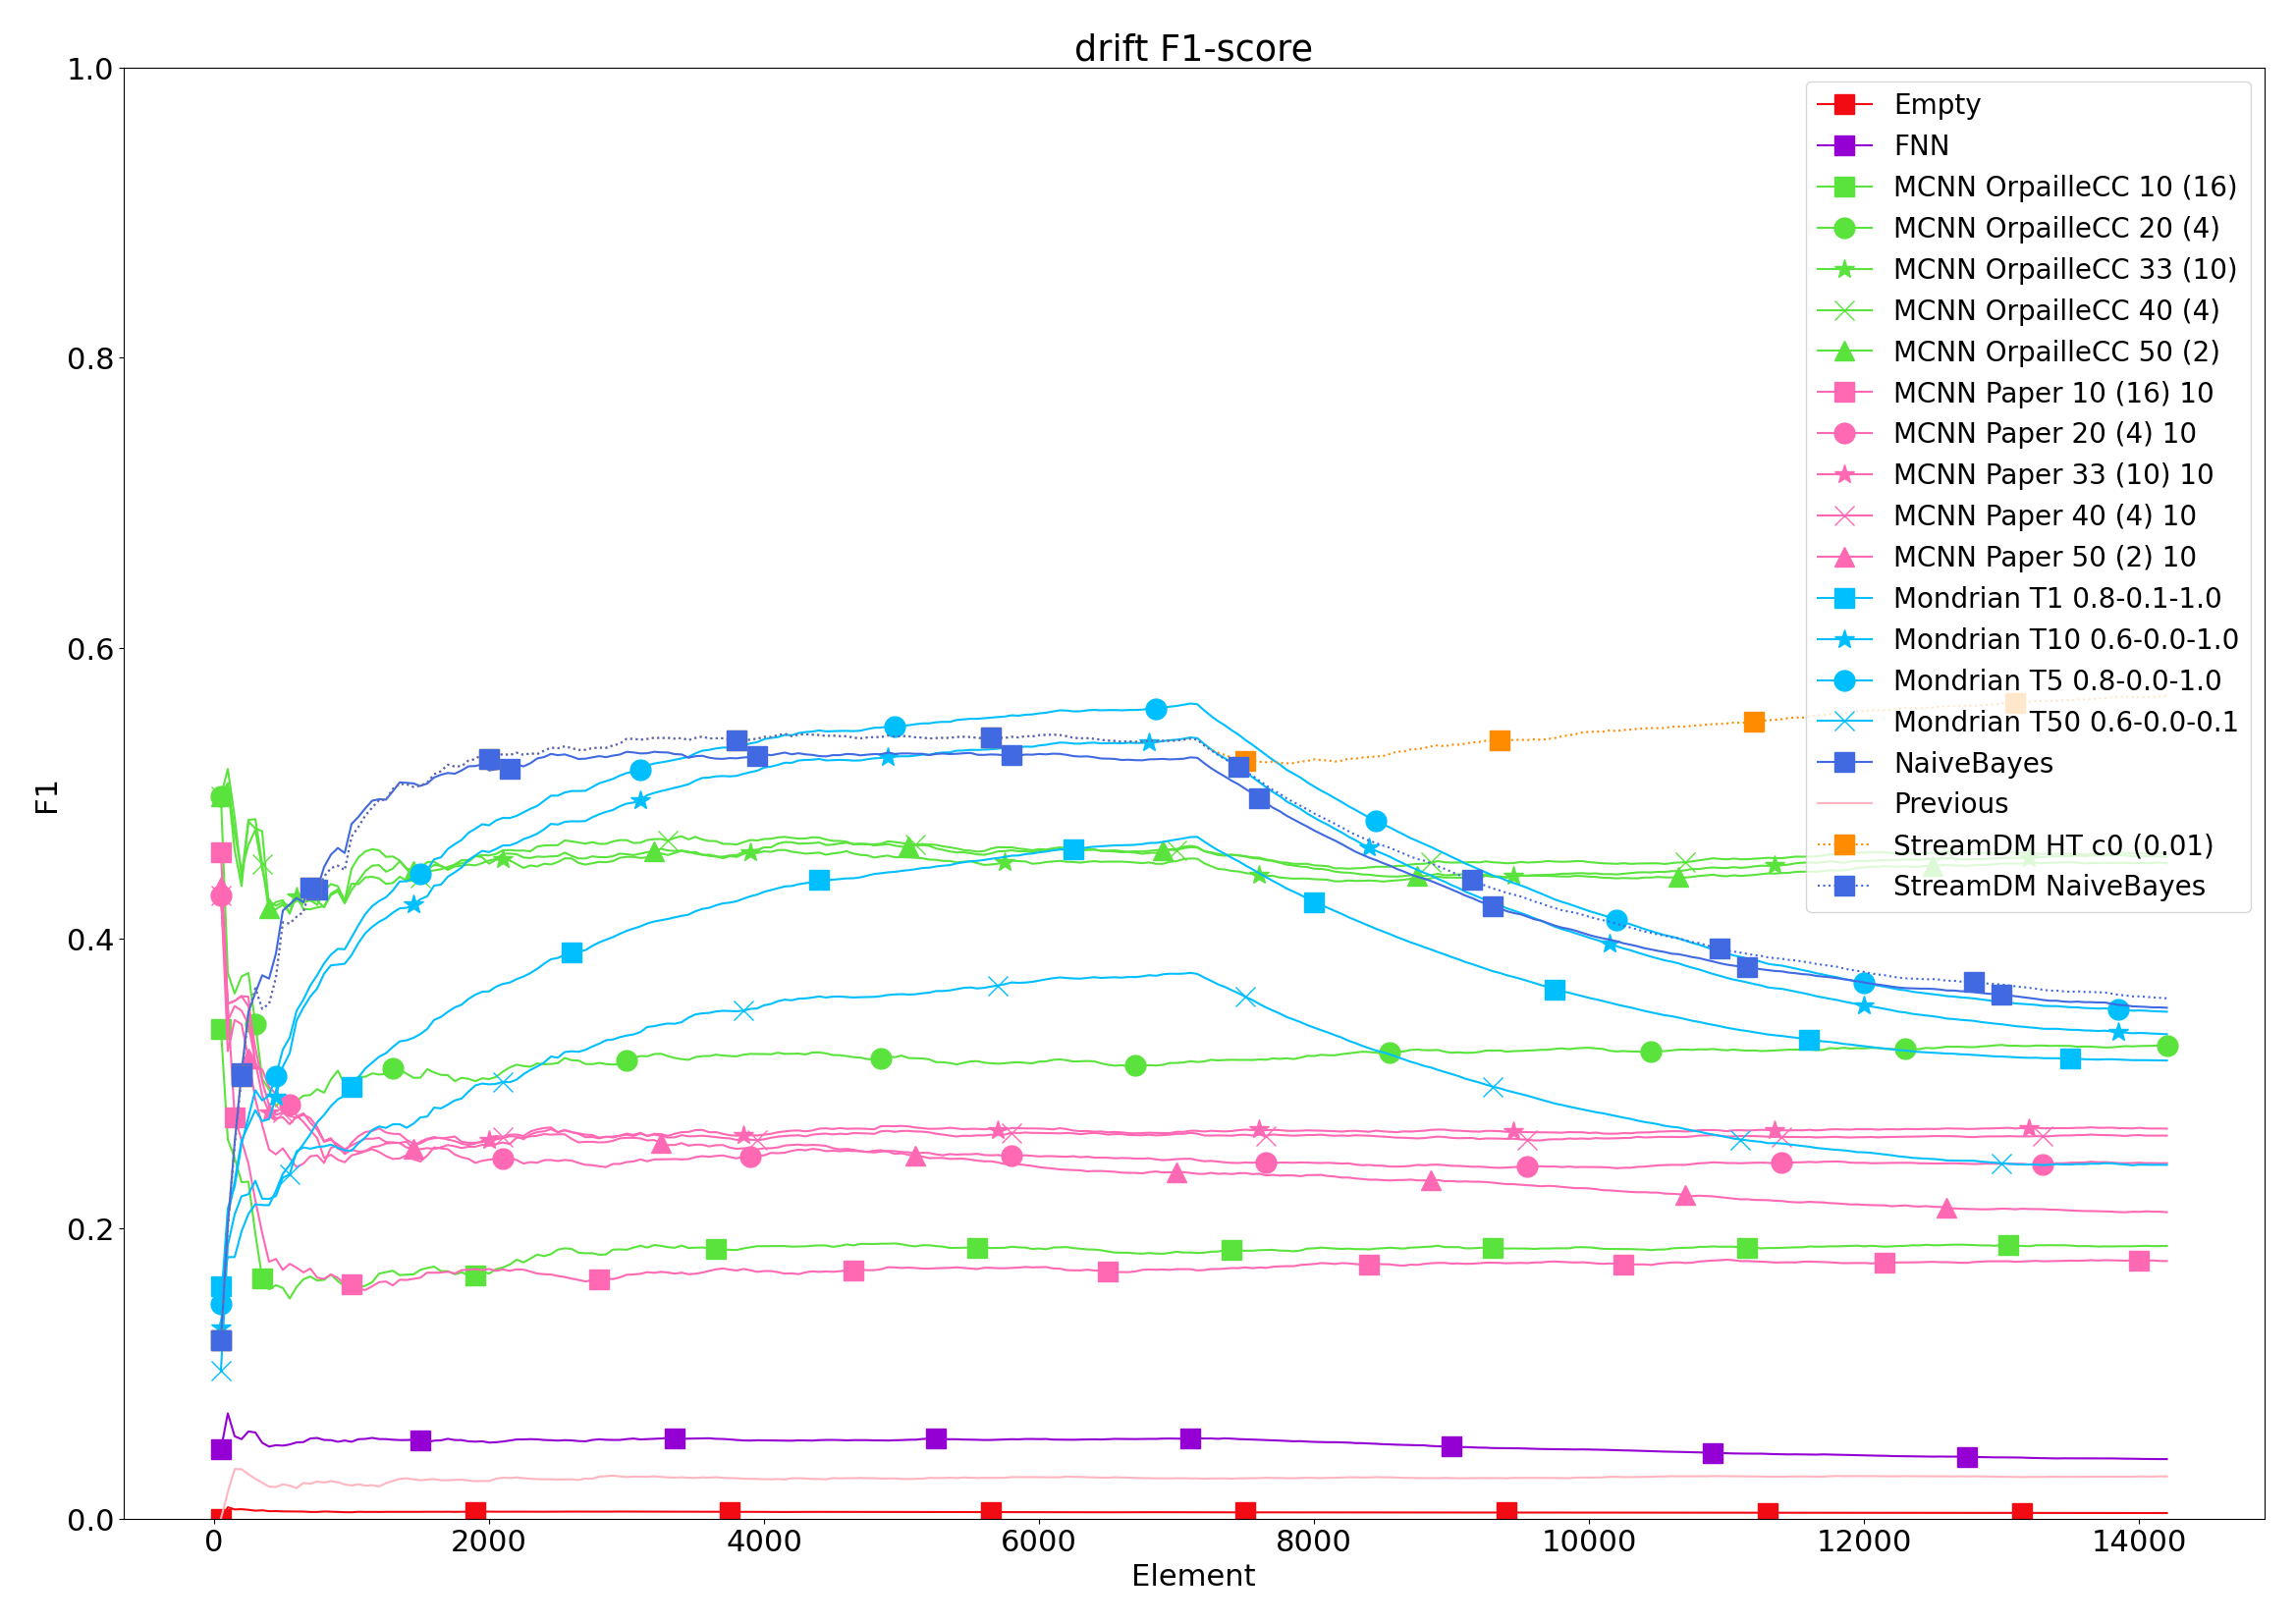
\includegraphics[width=\linewidth]{figures/results/drift_f1.png}
		\caption{Drift}
		\label{fig:f1-drift}
	\end{subfigure}
	\caption{F1-scores for the six datasets. \TG{remove titles on top of figures, they are redundant with captions}
	\TG{I would call ``Drift'' ``Banos et al (with drift)'' and put it in (b). I'd rename Hyperplane and the other MOA datasets to Hyperplane (MOA), etc }
	\TG{Hoeffding Tree is a bit difficult to see because it doesn't have a marker and the colour is a bit pale}
	\TG{You should explain what the MCNN and Mondrian params are, I think just adding ``trees'' (ex: ``10 trees'' and ``clusters'' (ex: ``10 clusters'' in the legend would be enough))}}
	\label{fig:f1}
\end{figure*}

\section{Results}

This section presents the results of our benchmark and the corresponding
hyperparameter tunning experiments.

\subsection{F1-score}


Figure~\ref{fig:f1} compares the F1-scores obtained by all classifiers on the six datasets. 
 Mondrian Forests \TG{shall we call them ``Mondrian Forest'' consistently throughout the paper? 
Currently they are also called ``Mondrian Trees'' or just ``Mondrian''} with 5 or 10 trees achieve the best
asymptotical F1-score for 4/6 datasets, while the Hoeffding Tree is the best-performing classifier for 2/6 datasets.

F1-score values vary greatly across the datasets.  While the highest
observed F1-score is above 0.95 on the Hyperplane and RandomRBF datasets,
it barely reaches 0.6 for the \banosdataset dataset, and it remains under
0.3 on the \recofitdataset and RandomTree datasets. This trend is
consistent for all classifiers.

The StreamDM HoeffdingTree algorithm remains close to the StreamDM Naive Bayes \TG{Not really for all datasets, a finer description is required here.}.
It happens because the HoeffdingTree
uses a naïve Bayes in the leaves. However, we notice that the two start
diverging because the HoeffdingTree improves by reshaping its tree structure.
This is caused by either a sufficient amount of element or by a drift.

In Figure~\ref{fig:f1-banos}, there are two types of MCNN: MCNN-Origin and
MCNN-OrpailleCC.  Both algorithm are implemented in the library OrpailleCC,
however, MCNN-Origin strictly follows the algorithm described in~\cite{mc-nn}
whereas MCNN-OrpailleCC tweaks this algorithm to ensure a fixed memory
footprint. The difference appears on how micro-clusters are removed.
MCNN-Origin removes a micro-cluster when its participation falls below a
threshold given by the user while MCNN-OrpailleCC removes the micro-cluster with
the least participation when the maximum number of micro-cluster is reached and
a new micro-cluster has to be introduced. \TG{Remove this paragraph, this is methods.}

In all cases, MCNN OrpailleCC achieves
better performance than MCNN Original. Additionally, most of
the time, any MCNN-OrpailleCC performs better than all MCNN-Origin \TG{not sure I understand this sentence. Maybe add a brief explanation instead, ``presumably due to \ldots''}.

On the real datasets (\banosdataset and \recofitdataset), the
Naive Bayes classifier appears to be learning faster than the Mondrian Forest, although Mondrian Forests catch up
after a few thousand elements. Even though it is difficult to notice on most of
the datasets, we can see on \banosdataset that MCNN OrpailleCC leans faster
than the naïve Bayes when there are less than a thousand elements \TG{not really obvious, and I would move that to the comparison between Original and Orpaille in the previous paragraph}.

Surprisingly, a Mondrian Forest with 50 trees performs worse than with
5 or 10 trees. This is due to the fact that our
Mondrian Forest implementation forces a fixed memory footprint, which limits tree growth
when the allocated memory is full. Because 50 trees fill the
memory faster than 10 or 5 trees, the classifier adaptation is blocked faster,
when the trees have not learned enough from the data. However, when the memory
available is increased, using 50 trees achieves better F1-scores than using 10
trees \TG{we can't seem to see this in the figure, I think we should remove this last comment.}.

The Hoeffding Tree appears to be the most robust to concept drifts
(Figure~\ref{fig:f1-drift}), while the Mondrian Forests and Naive Bayes
classifier are the most impacted. MCNN classifiers sare marginally impacted.
The low resilience of Mondrian Forests to concept drifts can be attributed
to two factors. First, Mondrian Forests cannot change the parts of the tree that
already exist even though it can reshape the tree \TG{unclear, reformulate}. Second, when the
memory limit is reached, Mondrian Forests are not able to grow or reshape their structure anymore.
\TG{The memory constraint needs to be better explained in the methods as this is a critical concept here. See comments in Section II.}

Finally, we notice that the StreamDM and Orpaille CC implementations of Naive Bayes remain close on the two real
datasets: \banosdataset and \recofitdataset \TG{how about the other ones though?}. This suggests that the two
implementations are similar, but SreamDM implements additional mechanisms \TG{this is too vague}.

\TG{Paragraphs should be added to comment on :
\begin{itemize}
	\item neural networks
	\item HoeffdingTree on the random tree dataset
\end{itemize}}


\begin{figure*}
	\begin{subfigure}[t]{.49\linewidth}
		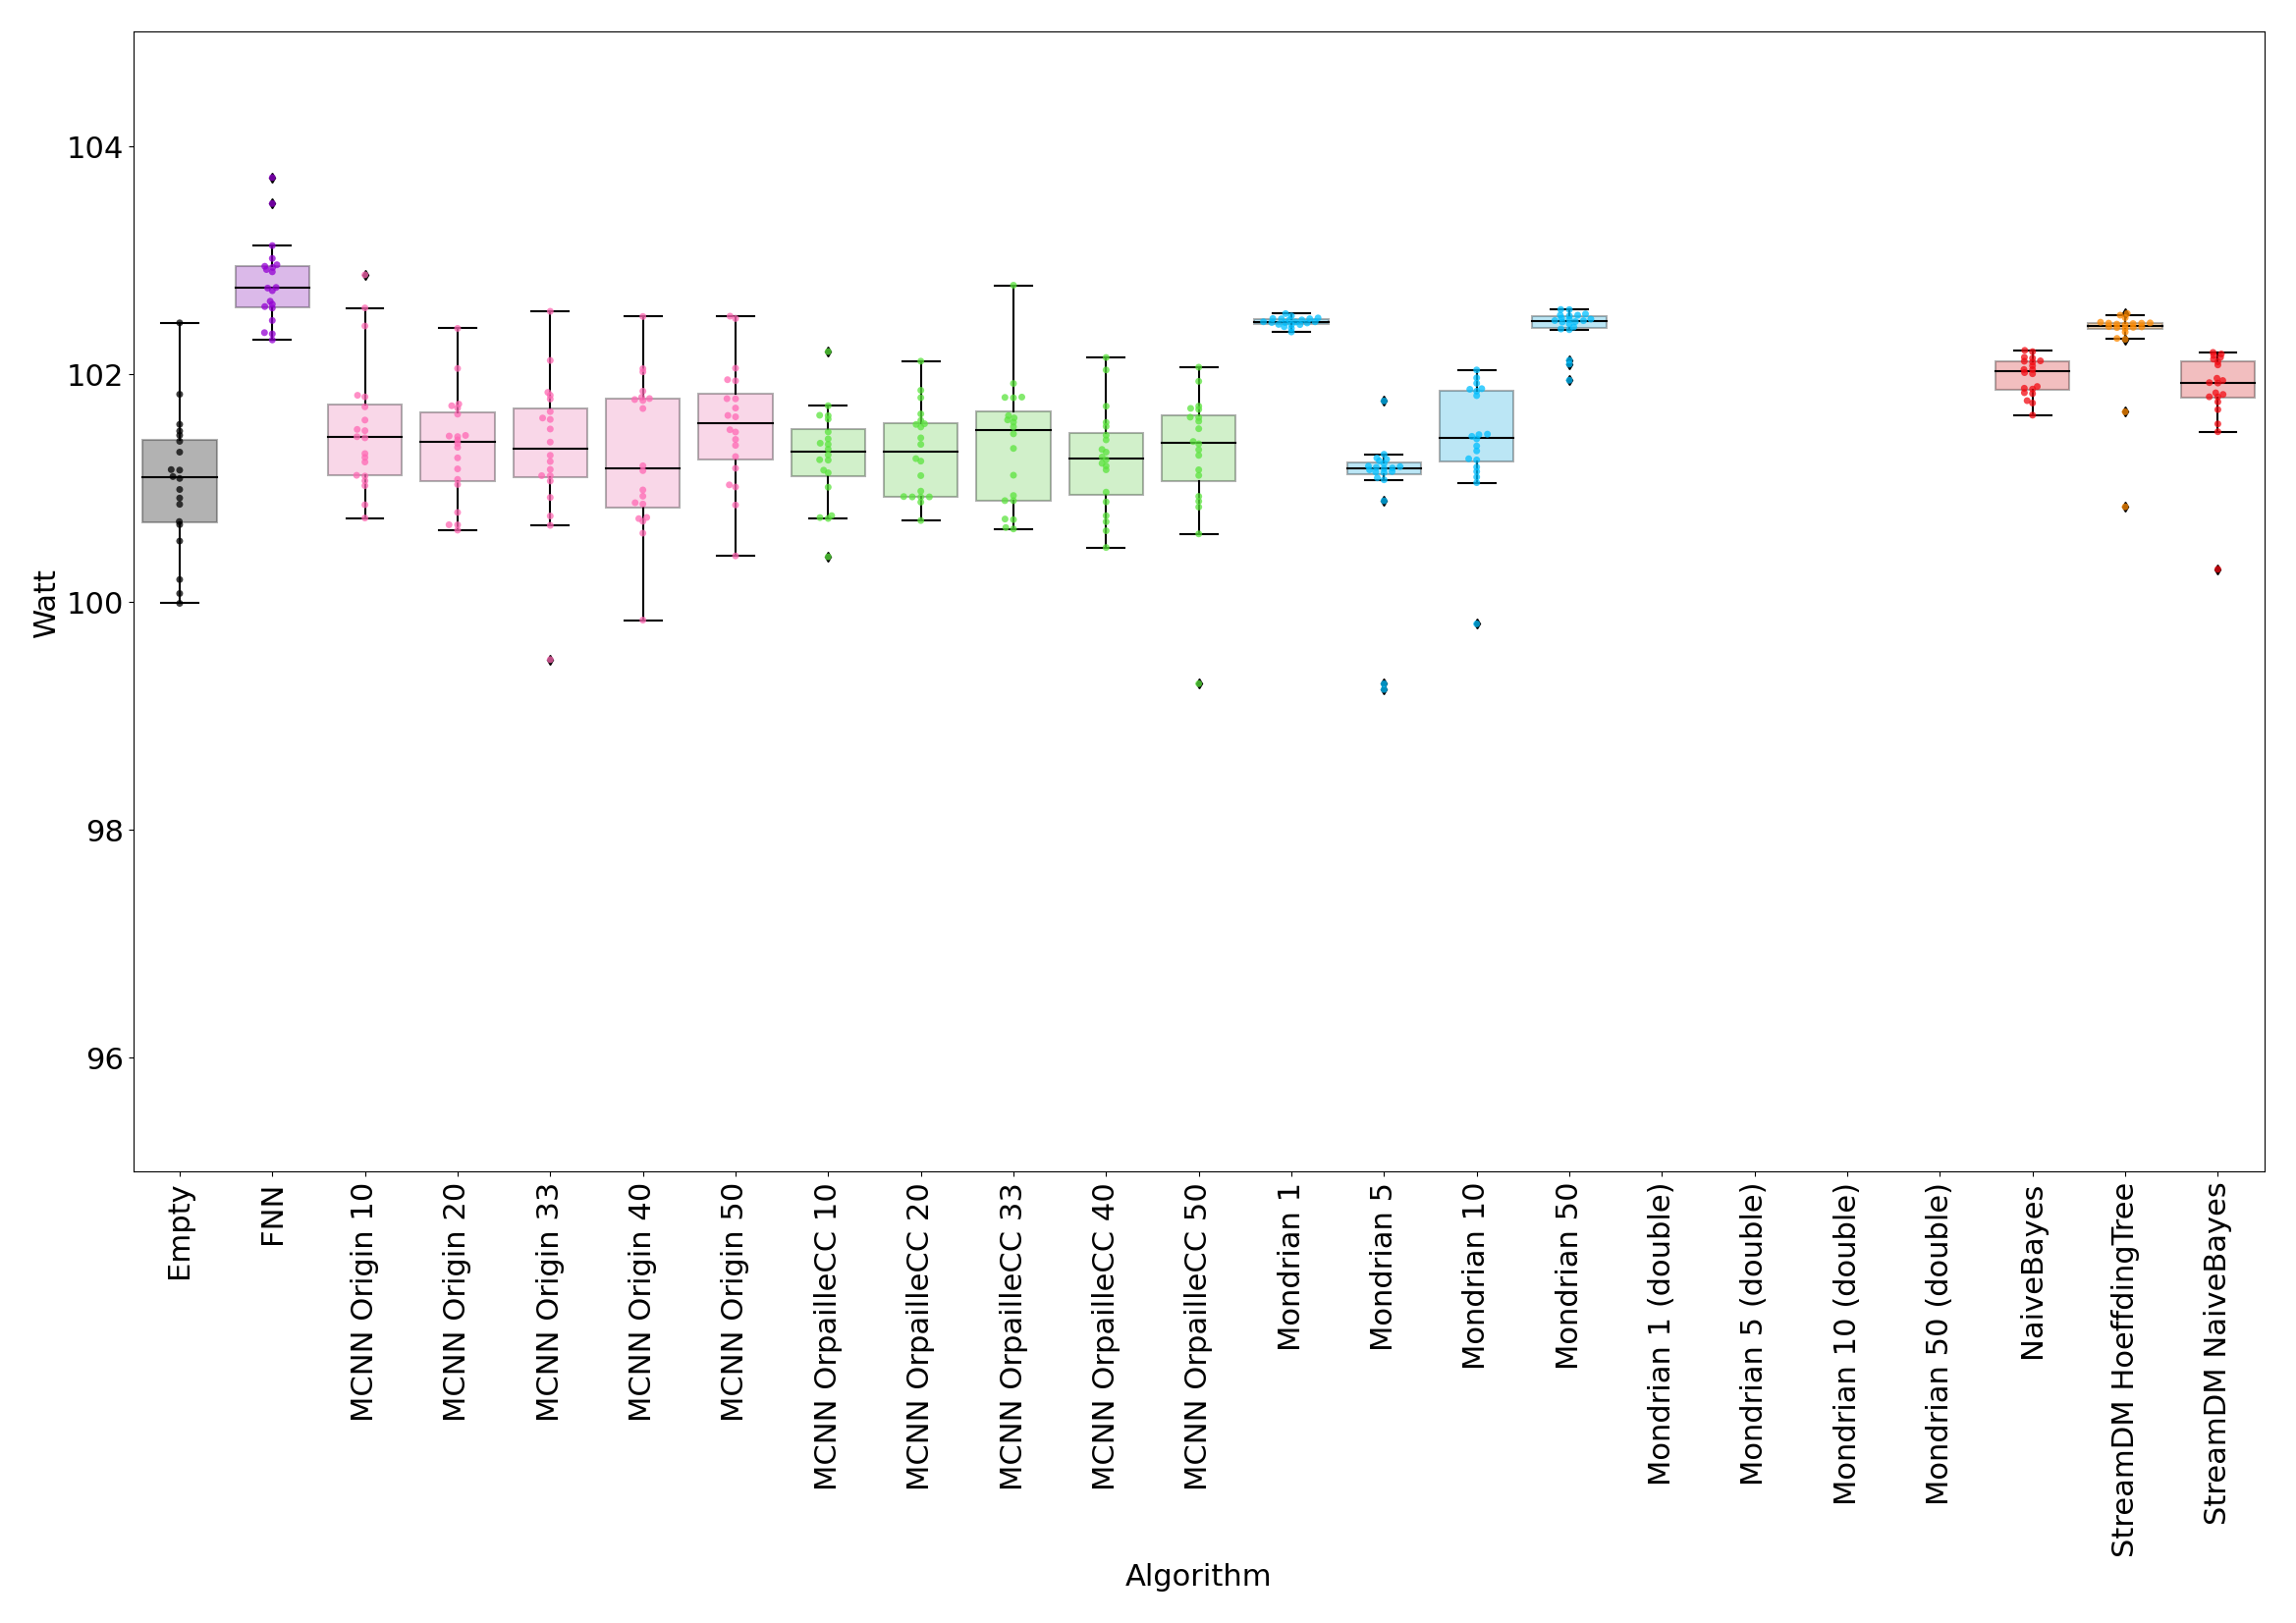
\includegraphics[width=\linewidth]{figures/results/banos_3_watt.png}
		\caption{\banosdataset}
		\label{fig:power-banos}
	\end{subfigure}
	\hfill
	\begin{subfigure}[t]{.49\linewidth}
		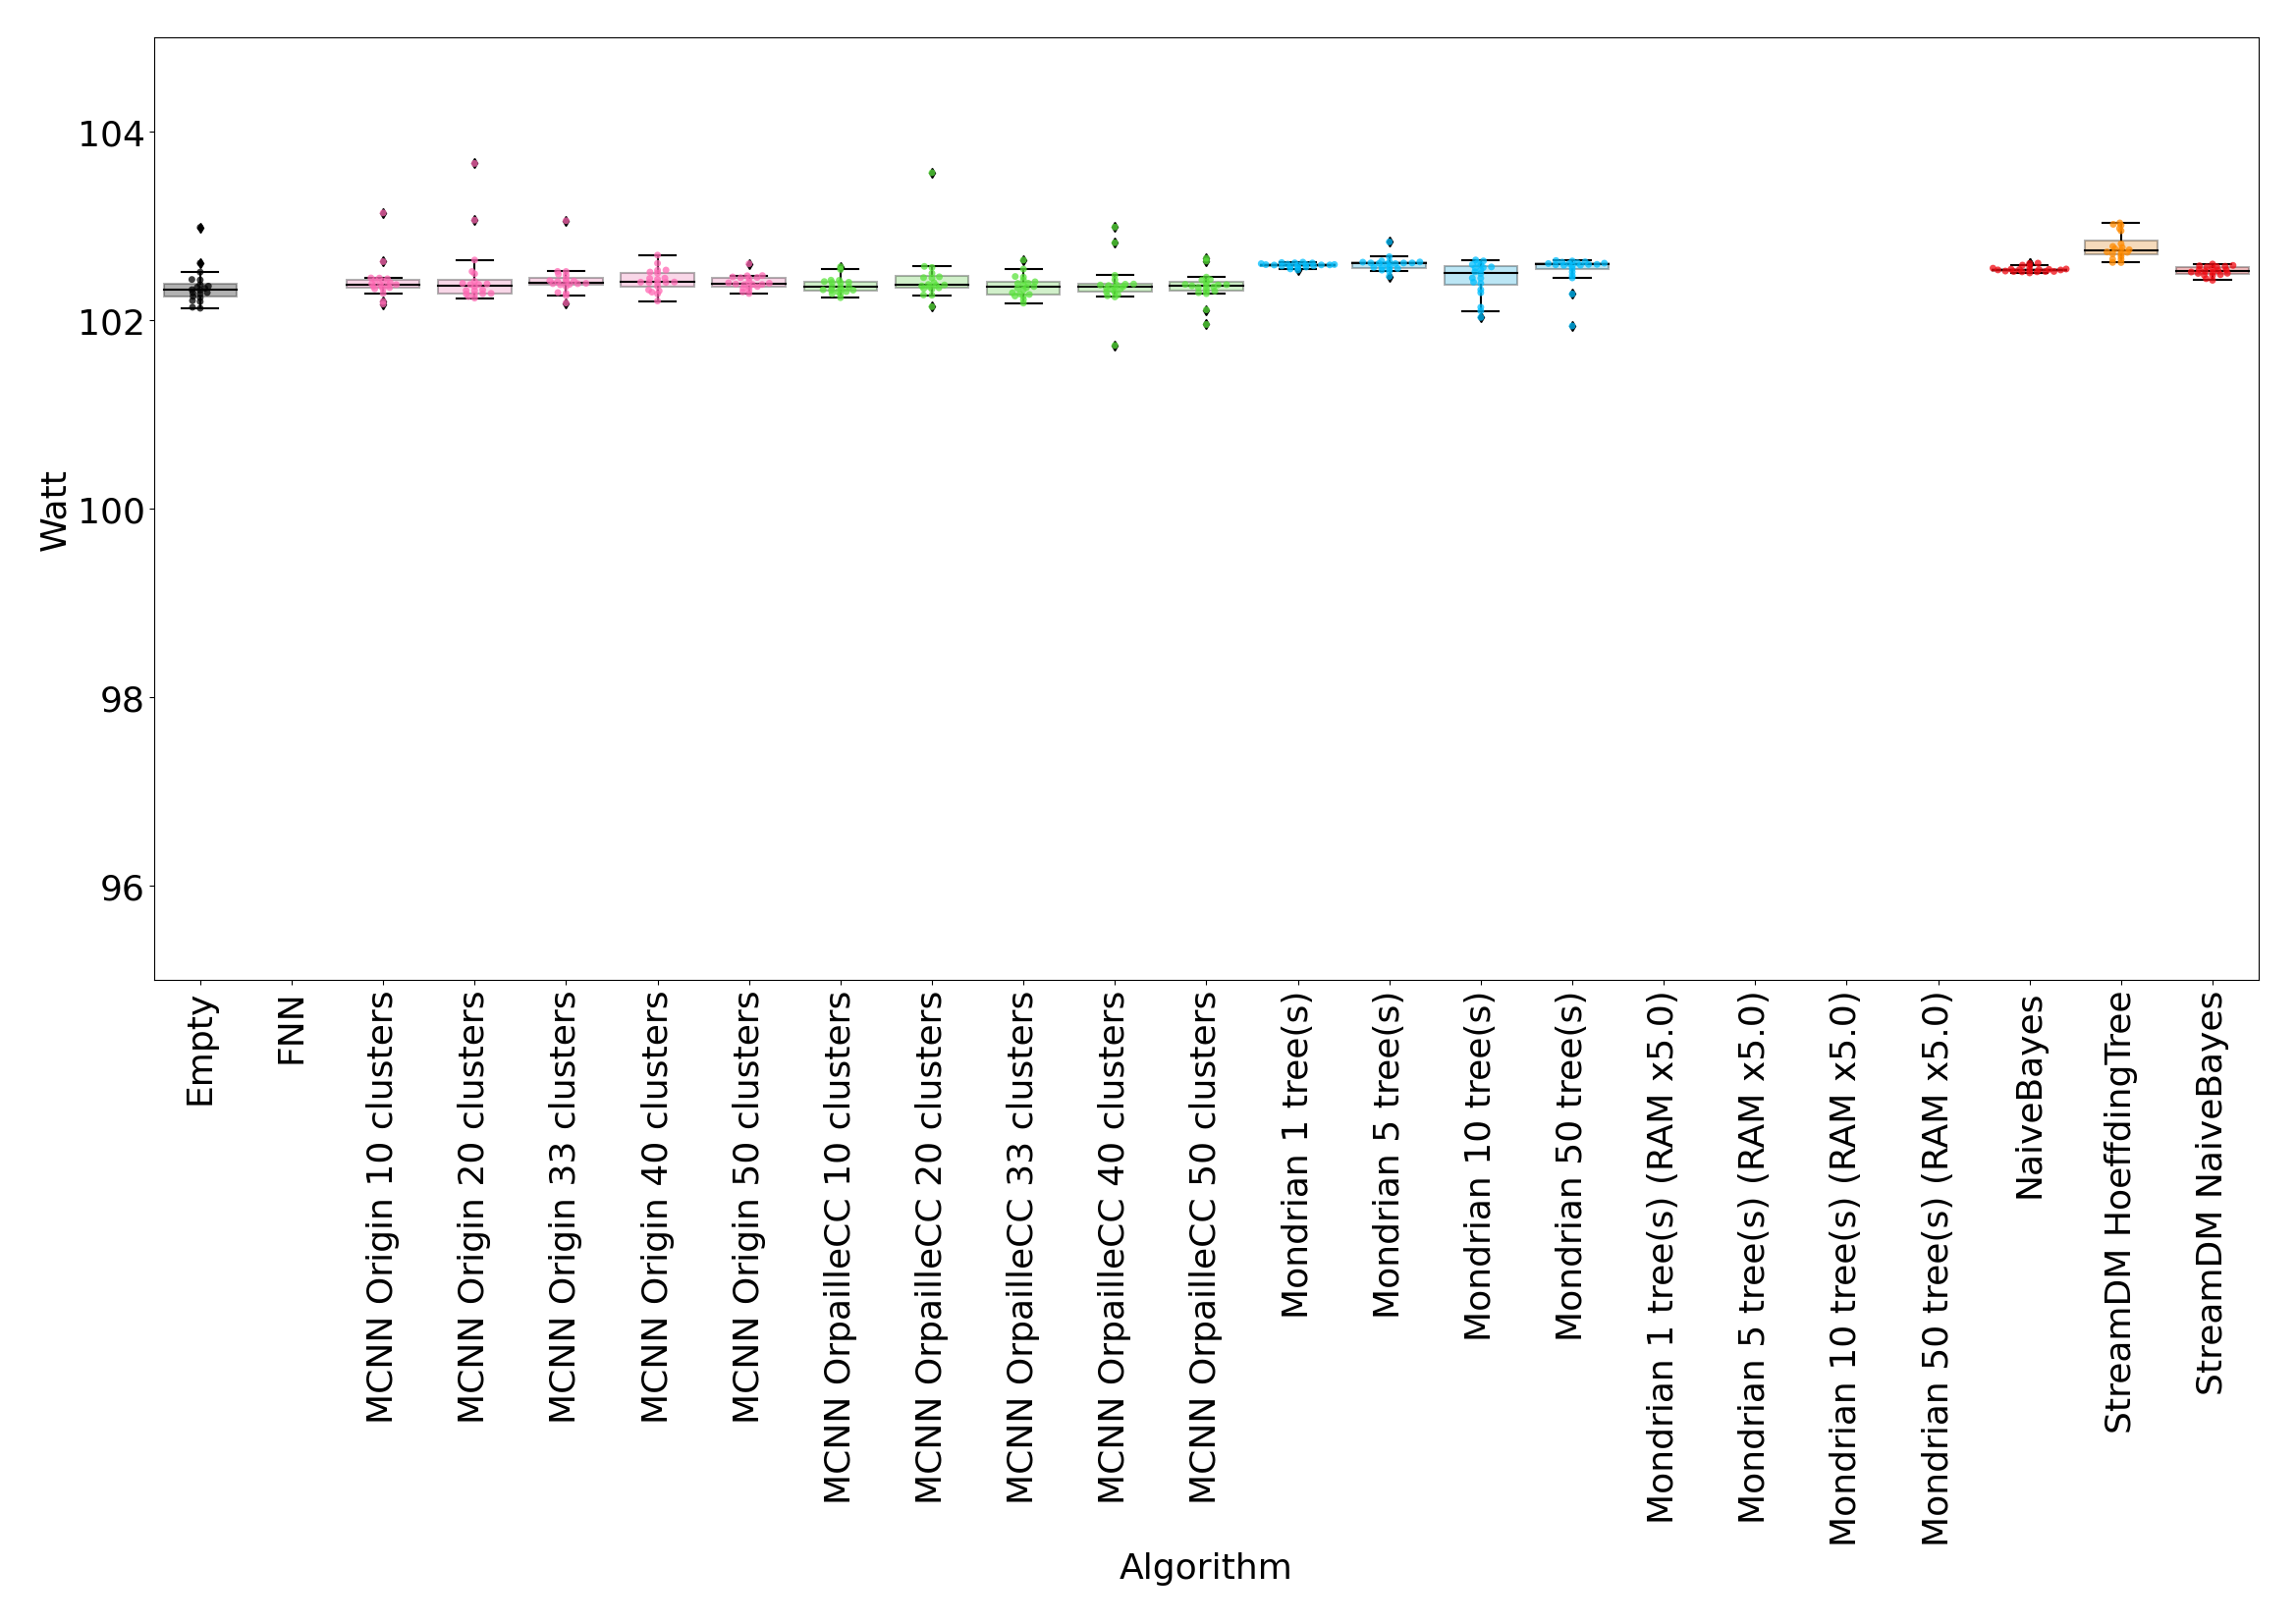
\includegraphics[width=\linewidth]{figures/results/recofit_3_watt.png}
		\caption{\recofitdataset}
		\label{fig:power-recofit}
	\end{subfigure}\\
	\begin{subfigure}[t]{.49\linewidth}
		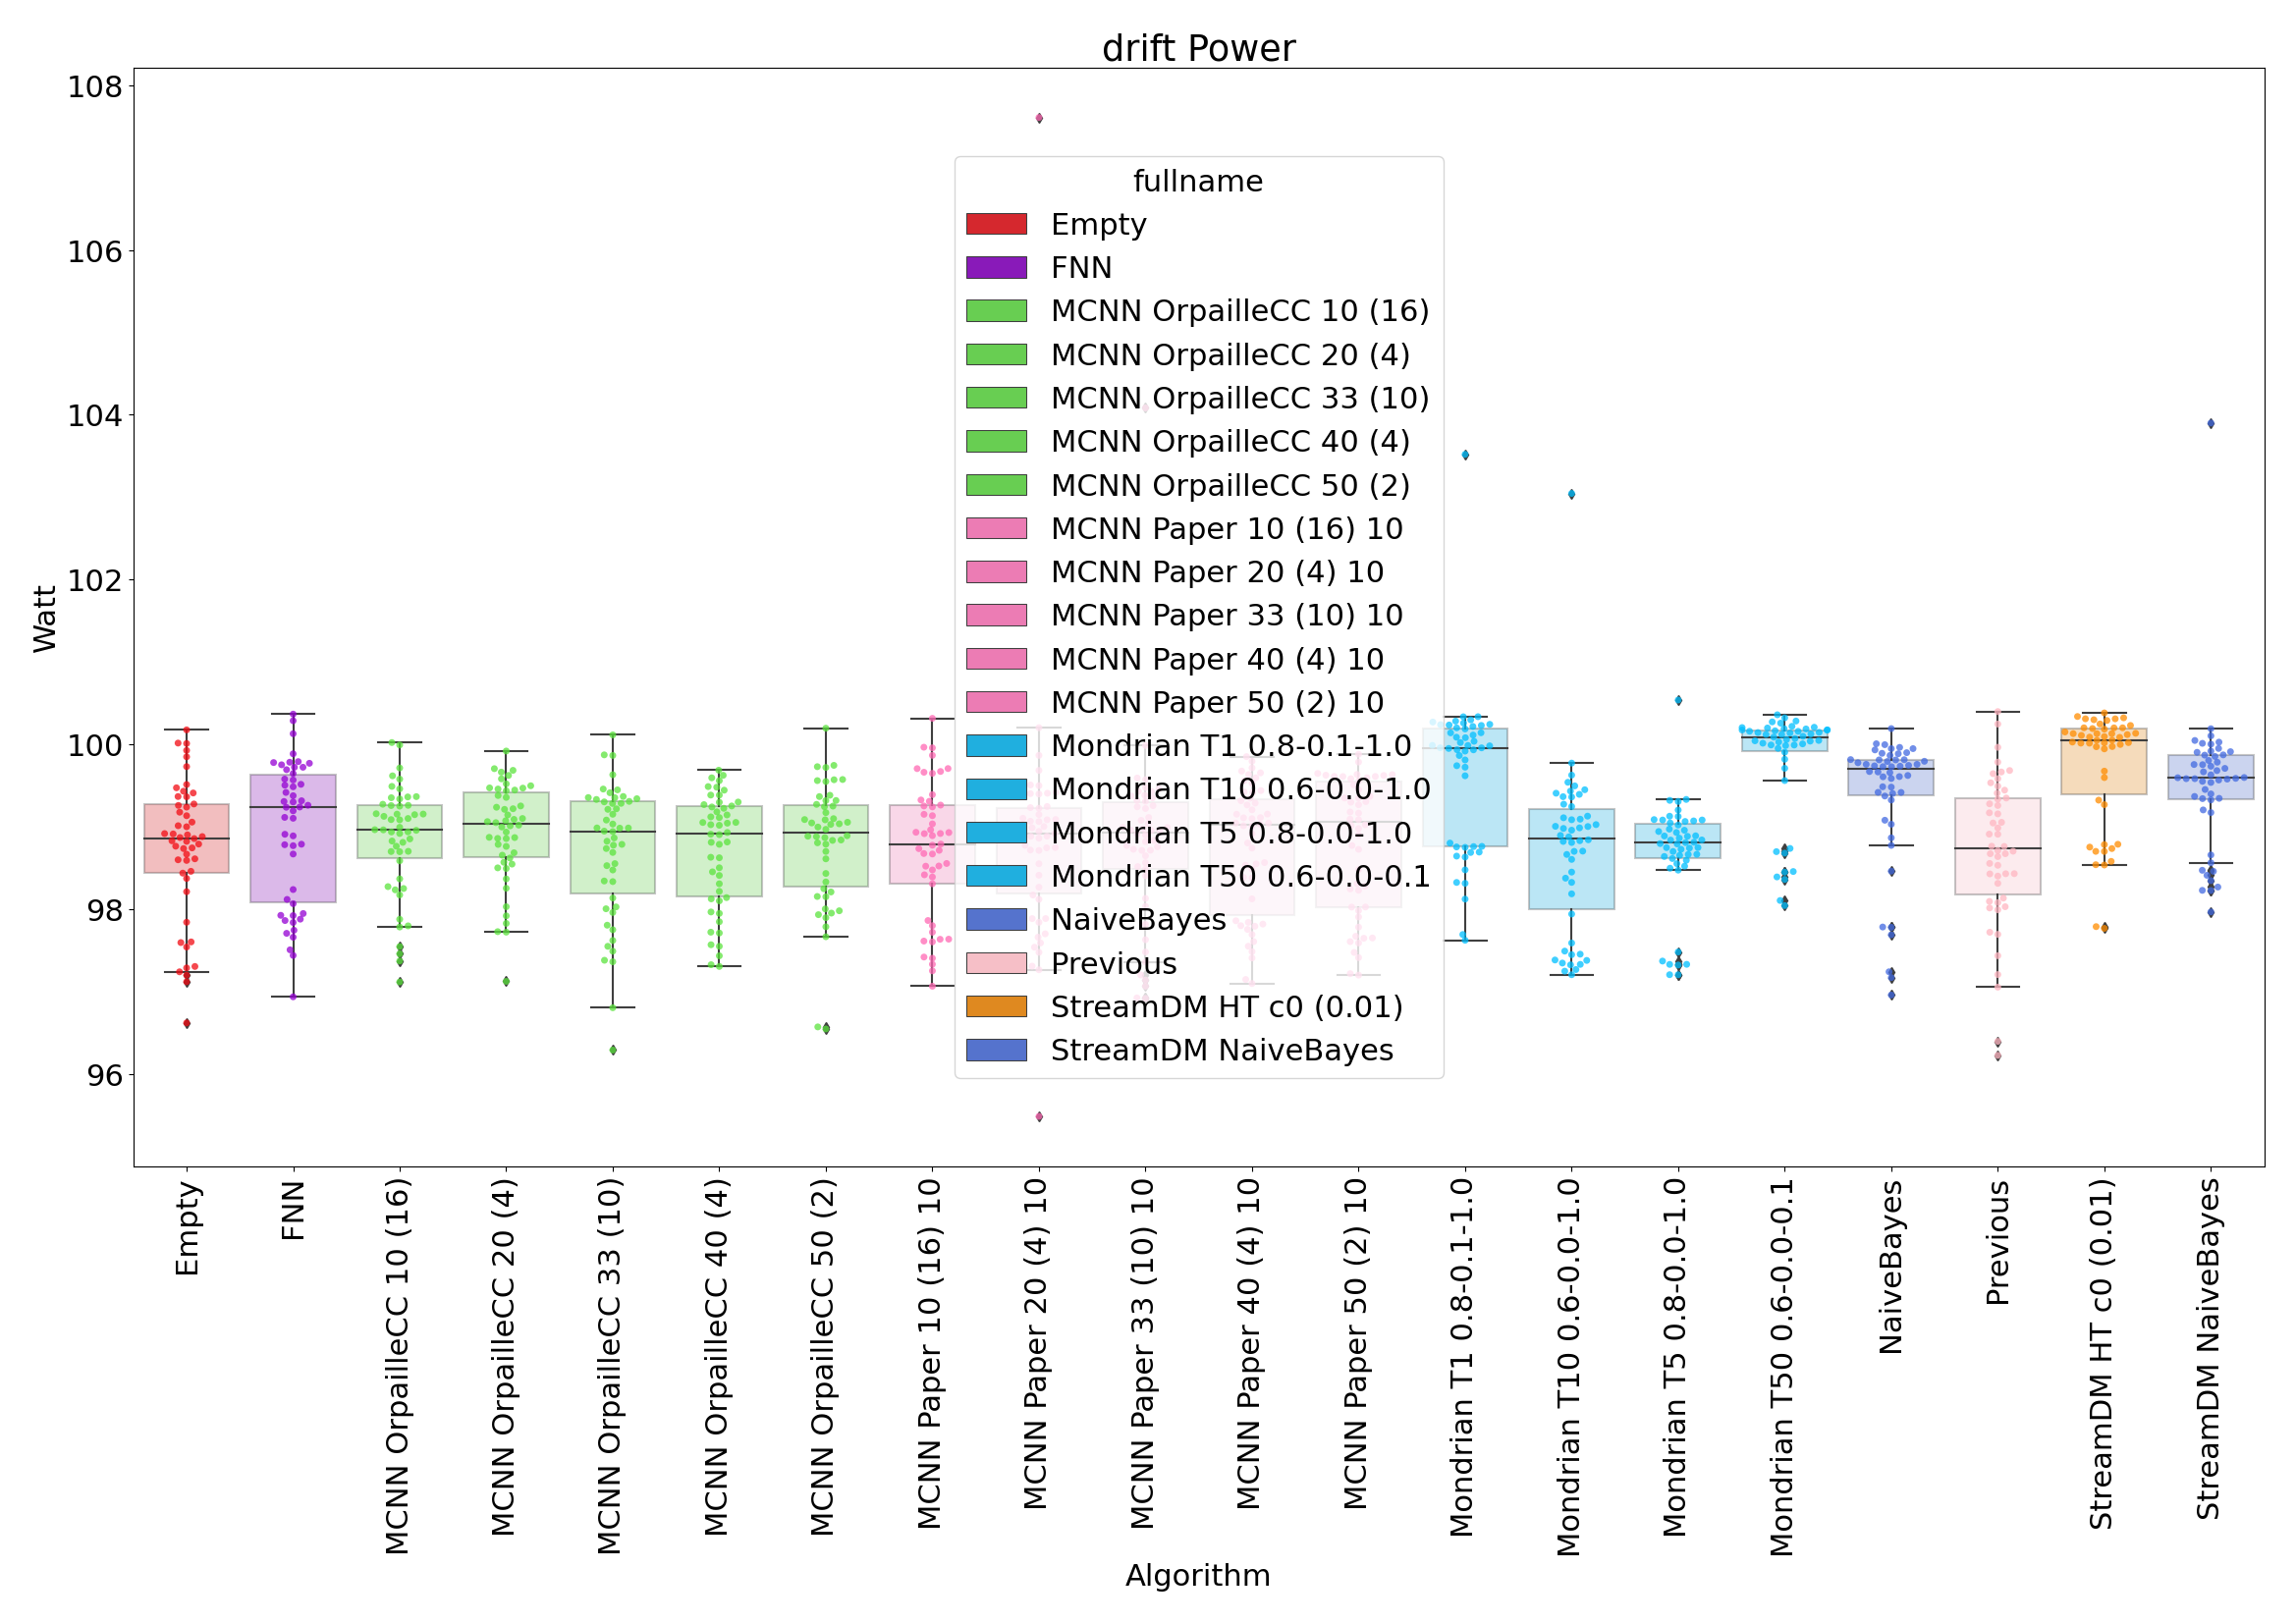
\includegraphics[width=\linewidth]{figures/results/drift_watt.png}
		\caption{\banosdataset with drift.}
		\label{fig:power-drift}
	\end{subfigure}
	\hfill
	\begin{subfigure}[t]{.49\linewidth}
		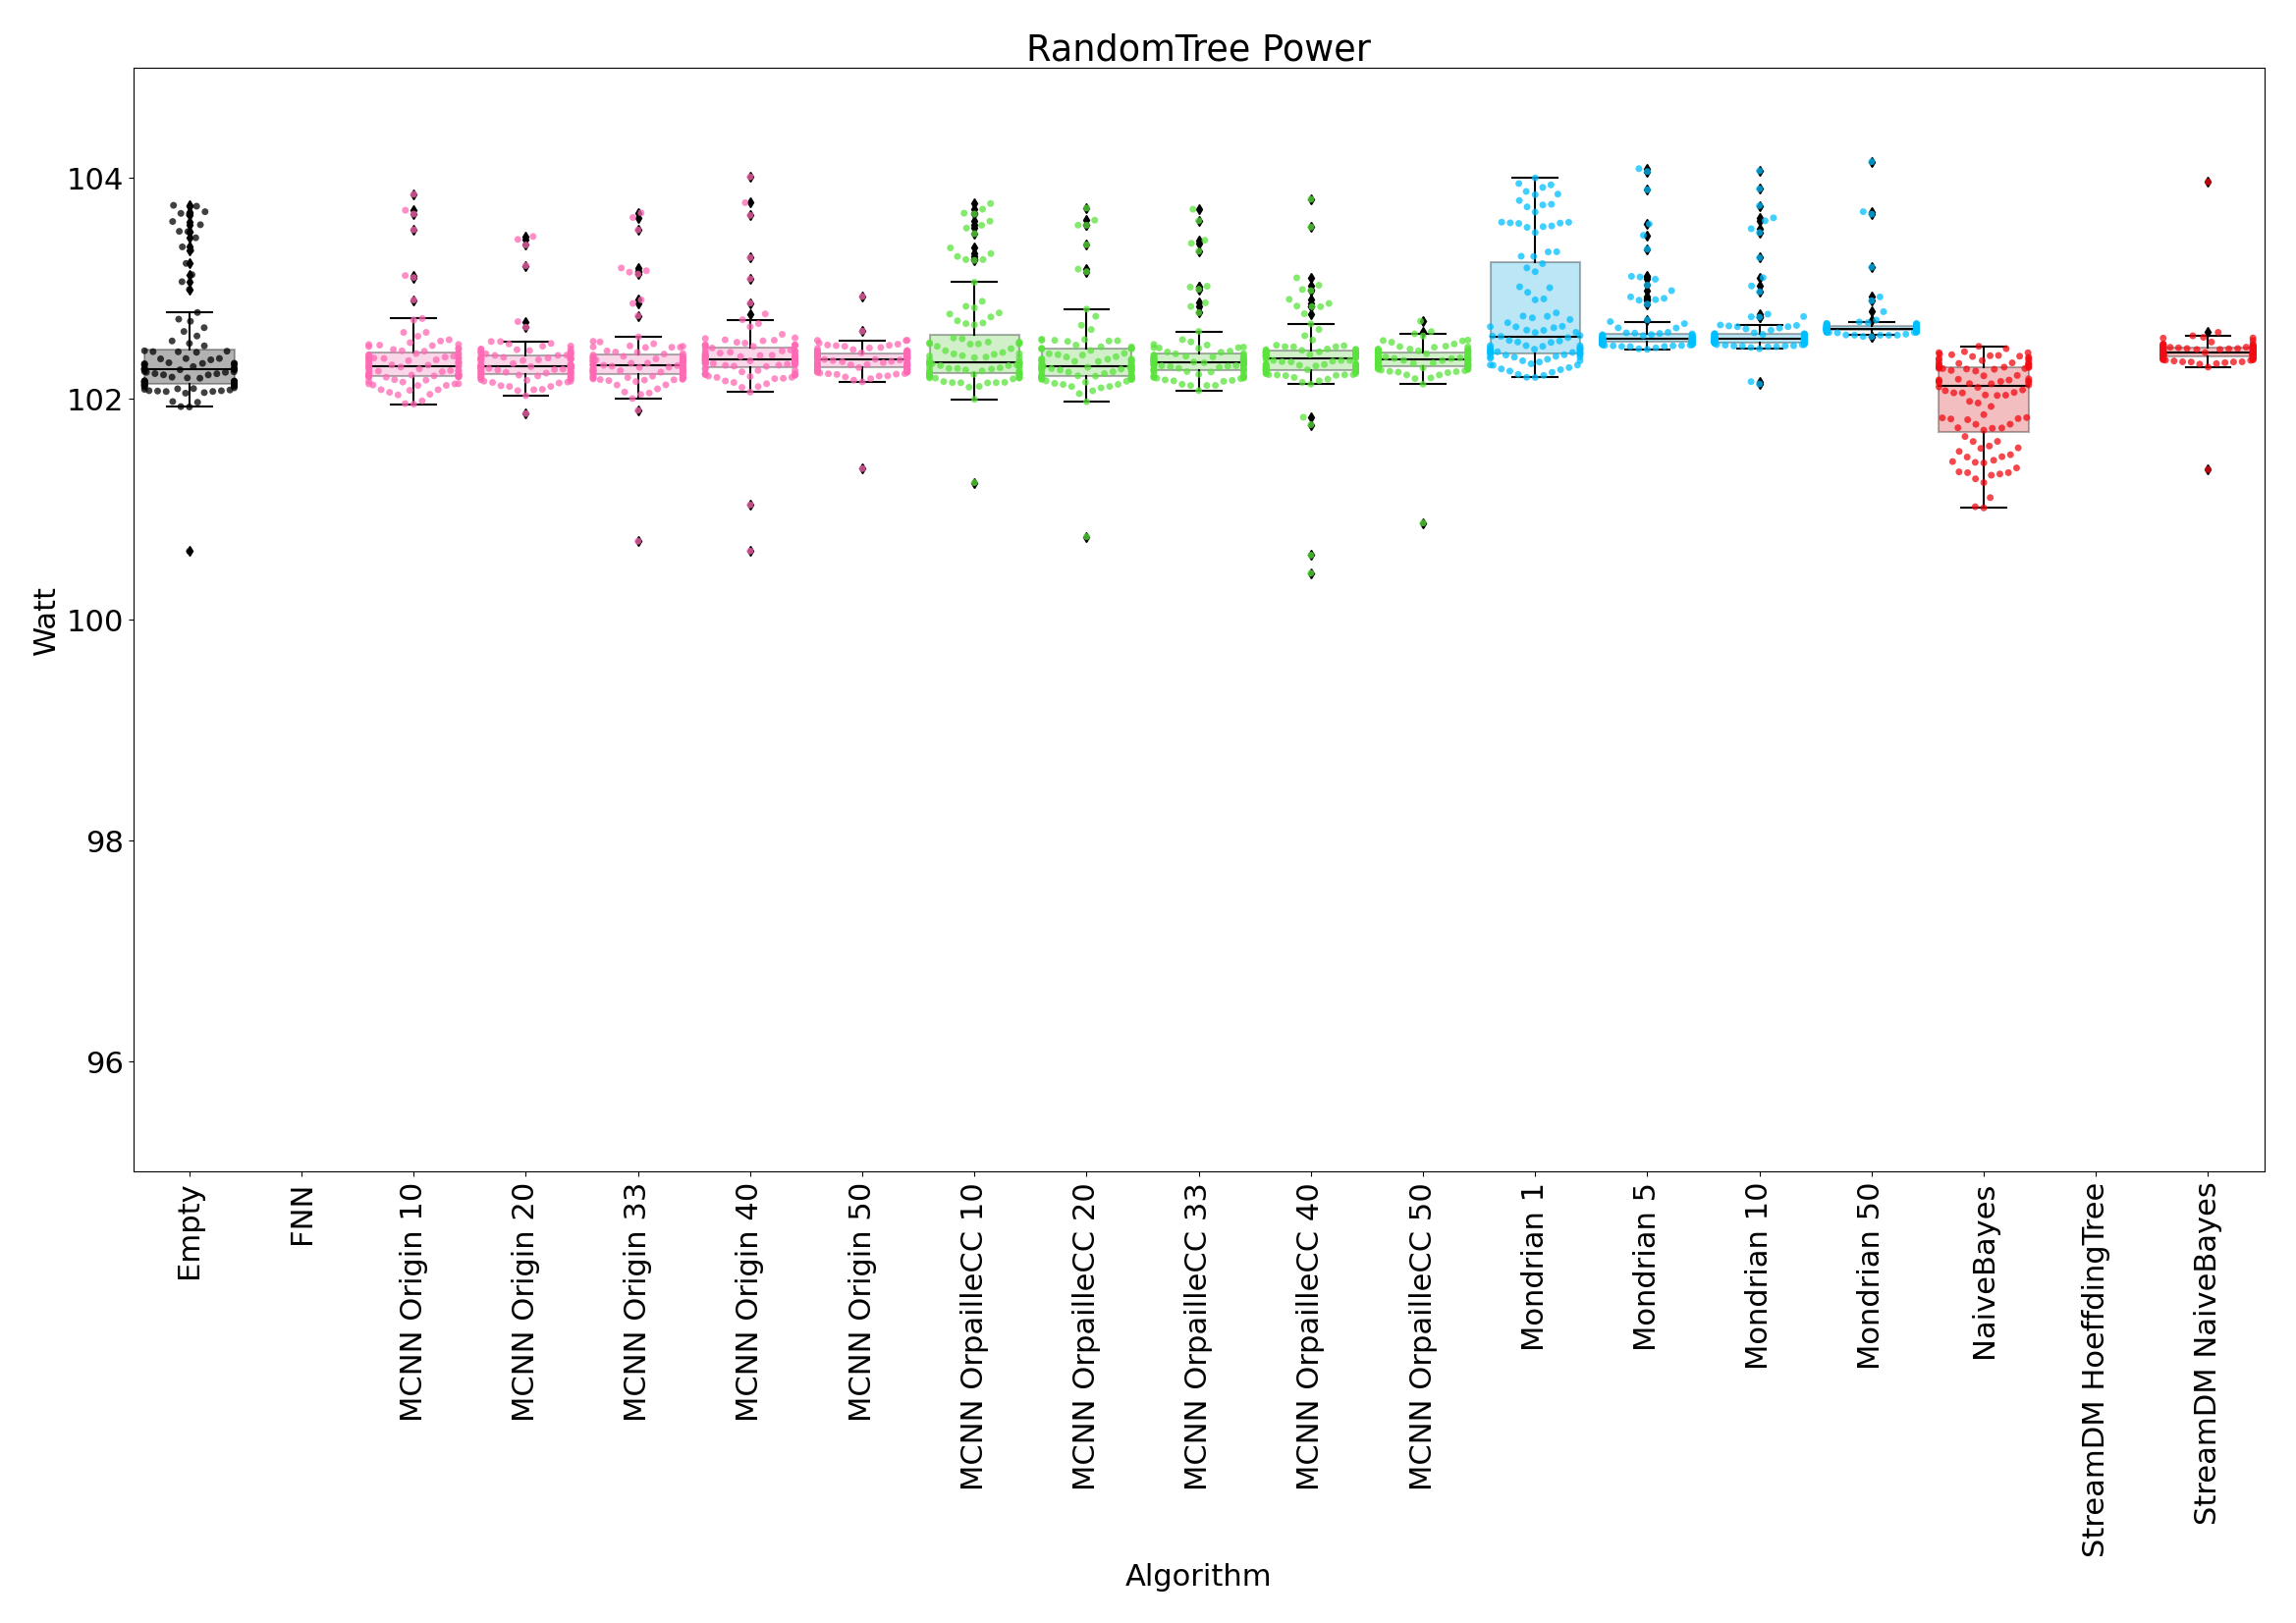
\includegraphics[width=\linewidth]{figures/results/dataset_3_watt.png}
		\caption{RandomTree}
		\label{fig:power-dataset_3}
	\end{subfigure}
	\caption{Power usage for four datasets.}
	\label{fig:power}
\end{figure*}
\subsection{Power}
\label{sec:result-power}
Figure~\ref{fig:power} shows the power usage of each classifier on four
datasets \TG{mention why the 6 datasets aren't reported}. All classifiers exhibit comparable power consumptions, close to 102~W.


\subsection{Runtime}
Figure~\ref{fig:runtime} shows the runtime of classifiers for the two real
datasets \TG{you haven't explained in the methods how runtime was
measured}. Mondrian Forests are the slowest classifier, in particular for
50 trees. The second slowest classifier is the Hoeffding Tree, which
compares with the 1-tree Mondrian Forest. The HoeffdingTree is followed by
the two Naive Bayes implementations, which is not surprising since Naive
Bayes classifiers are used in the leaves of the Hoeffding Tree. The MCNN
classifiers are the fastest ones, with a runtime very close to the empty
classifier. There is still a slight difference between the MCNNs. The more
cluster we use, the slower it gets \TG{at this scale it is barely
noticeable, I would ommit this comment.}.

We observe that naïve Bayes from StreamDM is slightly faster than the one
from OrpailleCC \TG{I think they are quite comparable in fact. You should
explain that this makes the comparison between hoeffding tree and mondrian
fair even though they are implemented differently.}.

\begin{figure*}
	\begin{subfigure}[t]{.49\linewidth}
		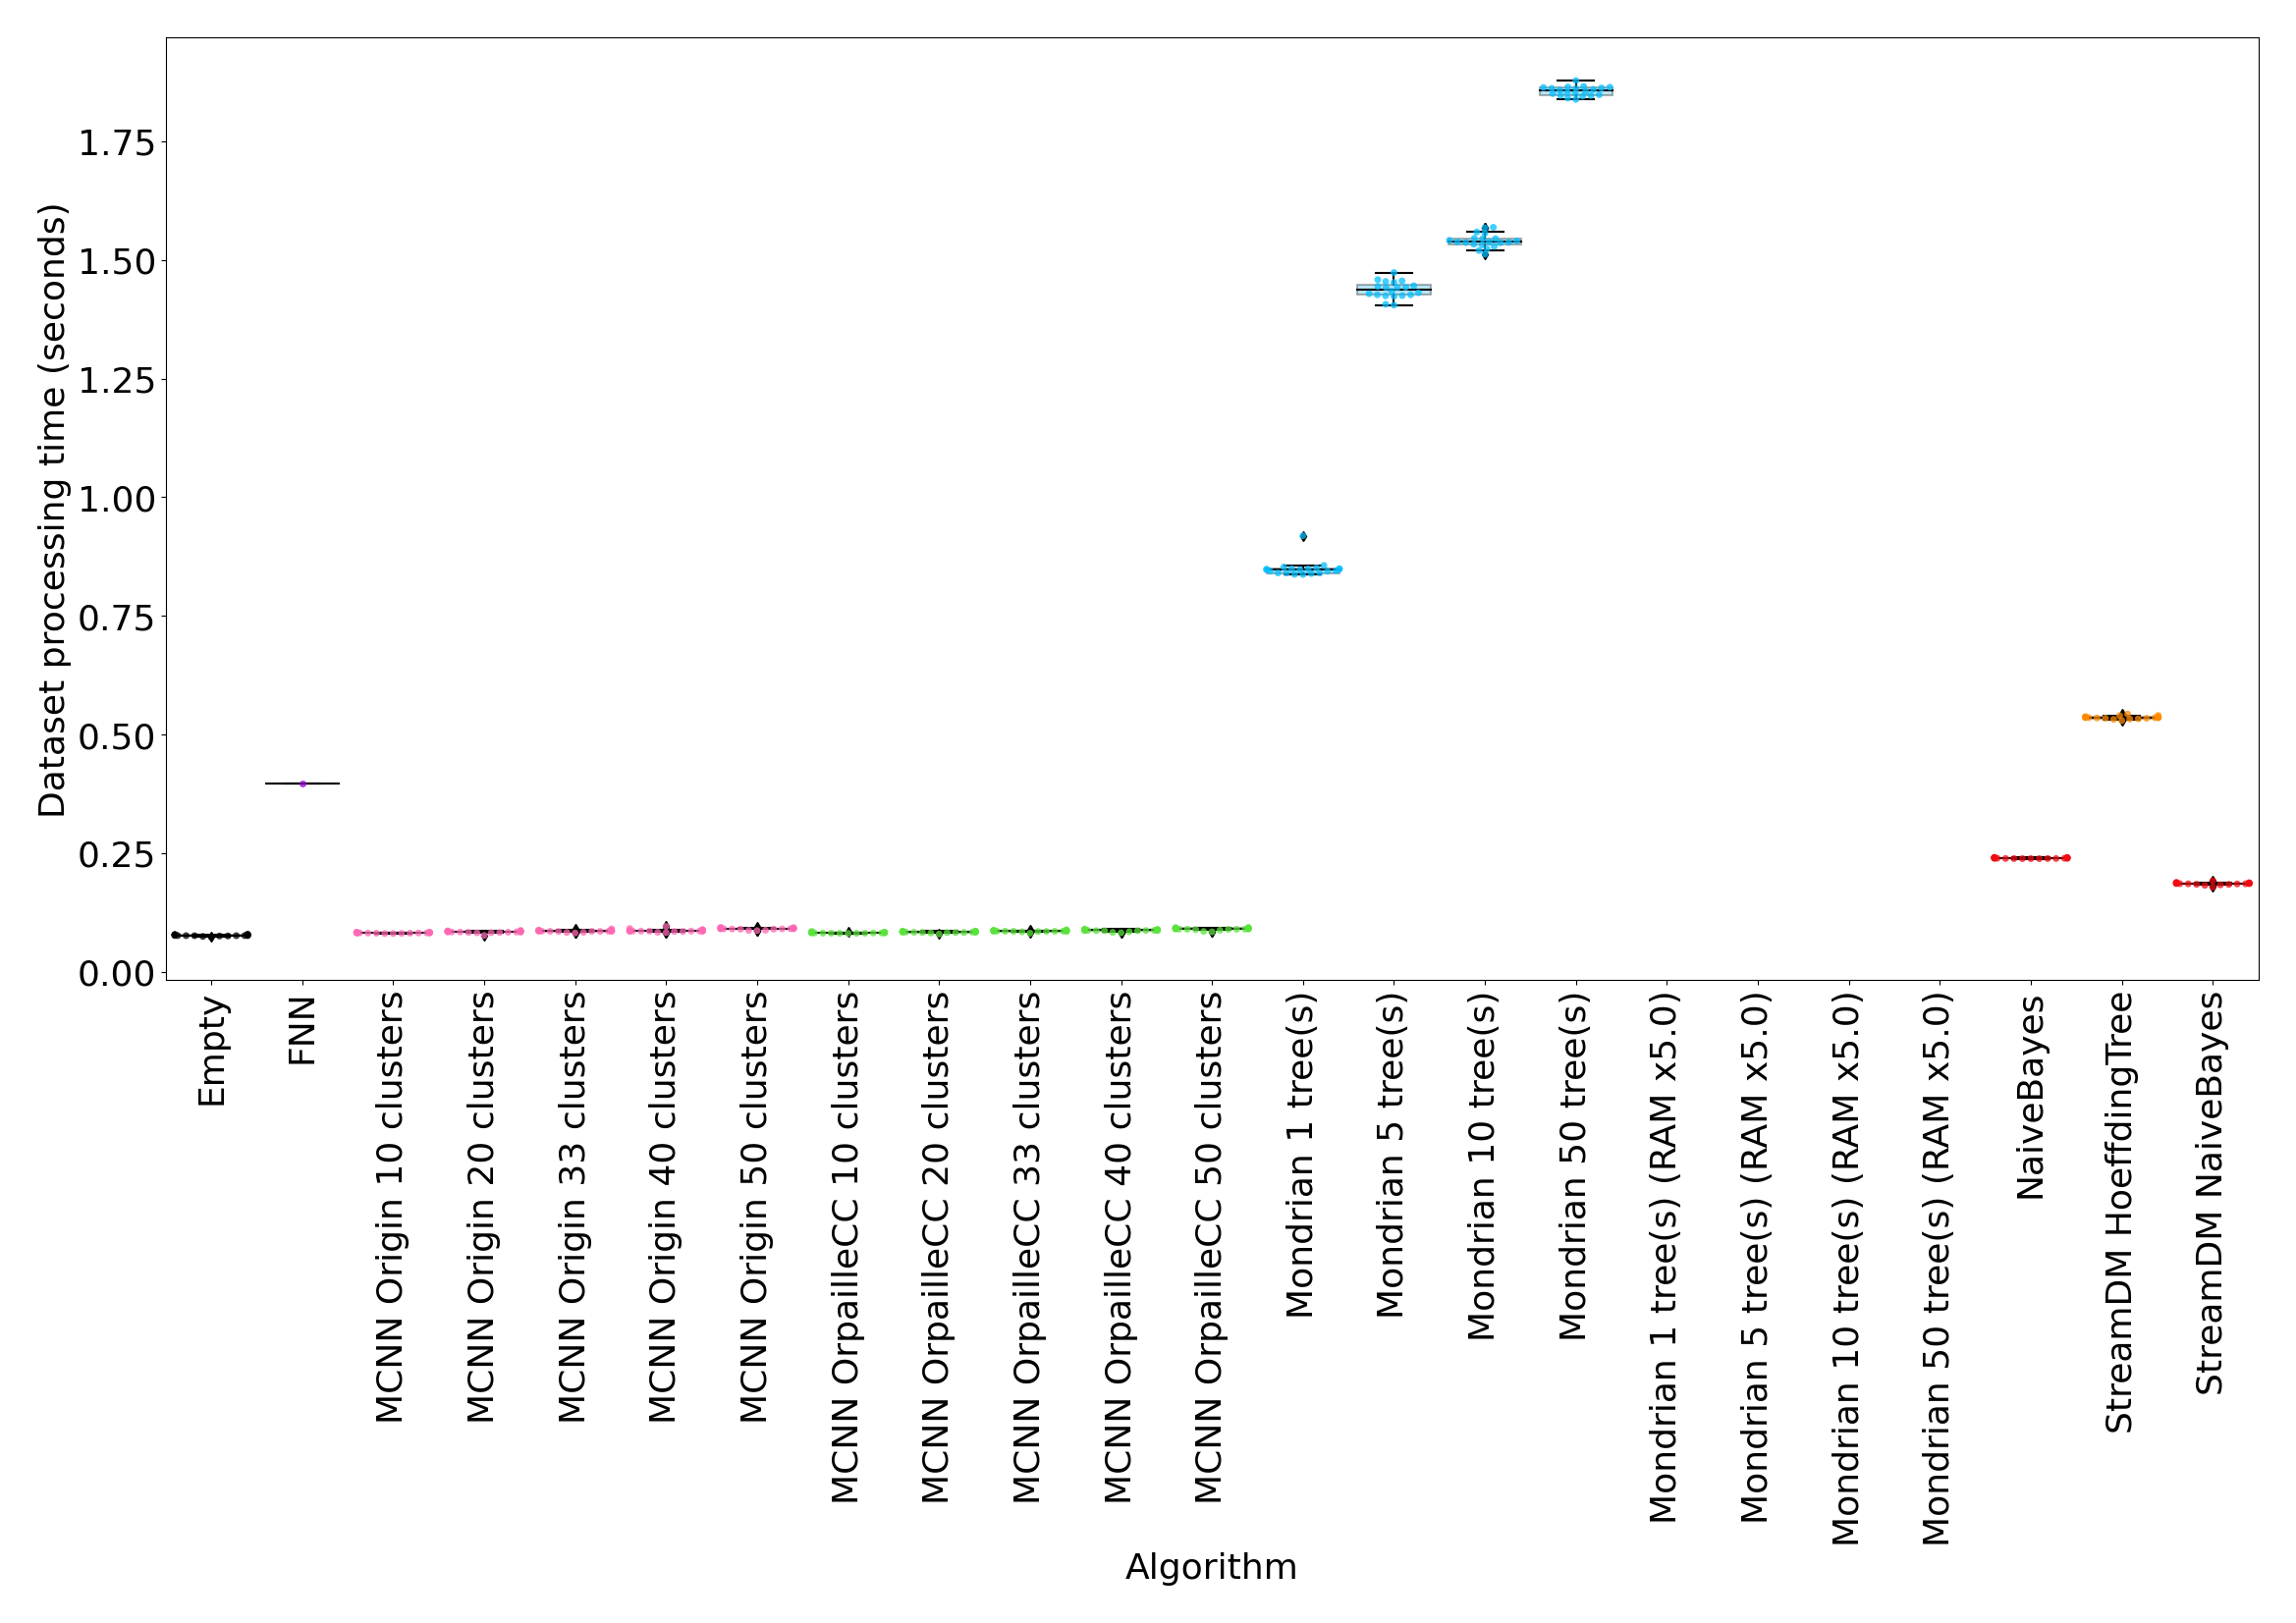
\includegraphics[width=\linewidth]{figures/results/banos_3_runtime.png}
		\caption{\banosdataset}
		\label{fig:runtime-banos}
	\end{subfigure}
	\hfill
	\begin{subfigure}[t]{.49\linewidth}
		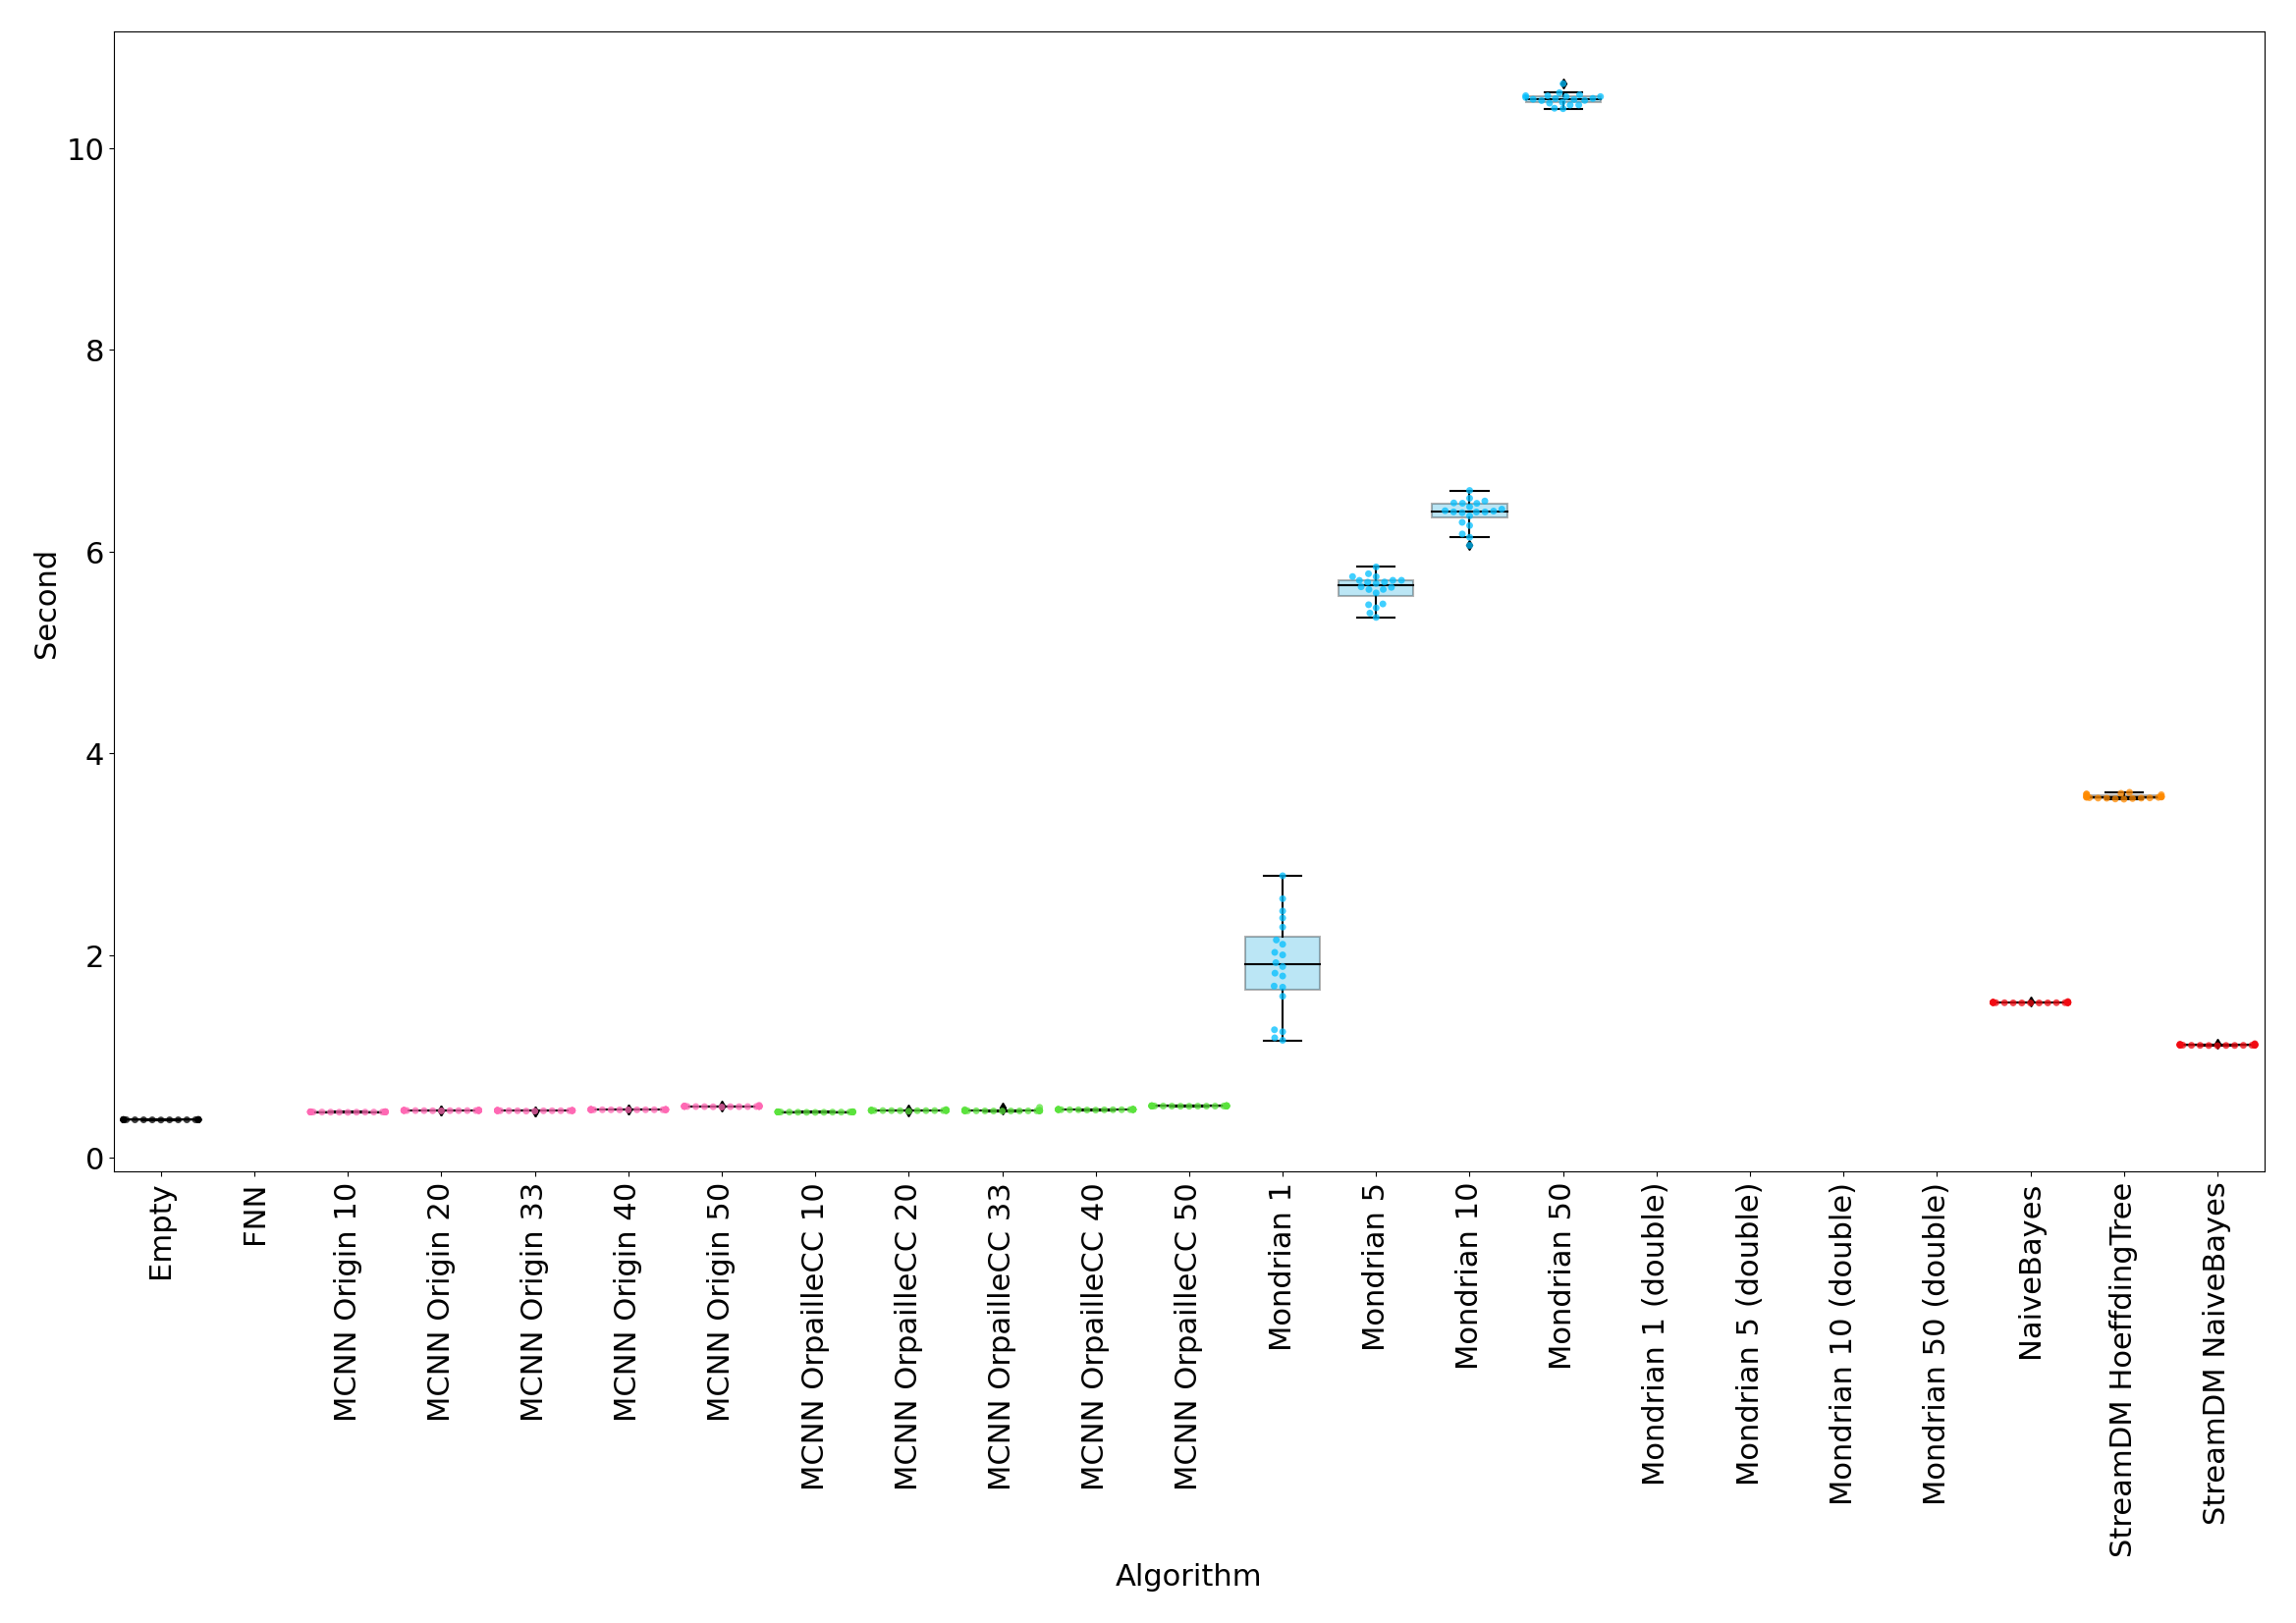
\includegraphics[width=\linewidth]{figures/results/recofit_3_runtime.png}
		\caption{\recofitdataset}
		\label{fig:runtime-recofit}
	\end{subfigure}
	\caption{Runtime with the two real datasets. \TG{y-axis should be ``Dataset processing time (seconds)''}}
	\label{fig:runtime}
\end{figure*}

\subsection{Memory}
\label{sec:result-memory}
Figure~\ref{fig:memory} shows the evolution of the memory footprint for the
\banosdataset dataset.  Memory footprint is similar across all datasets, due to the fact that most algorithms
follow a bounded memory policy or have a constant space complexity. The only
exception is the Hoeffding Tree \TG{check that spelling and capitalization
of Hoeffding Tree is consistent throughout document} that constantly
selects new splits depending on 
new data points. The Mondrian Forest would have had the same behavior if it
would allocate memory as element goes by. However, the Mondrian implementation
of OrpailleCC allocates memory when the classifier is instantiated and does not
use more \TG{Last two sentences should be improved, this can be written in a more compact way.}.

\begin{figure}
	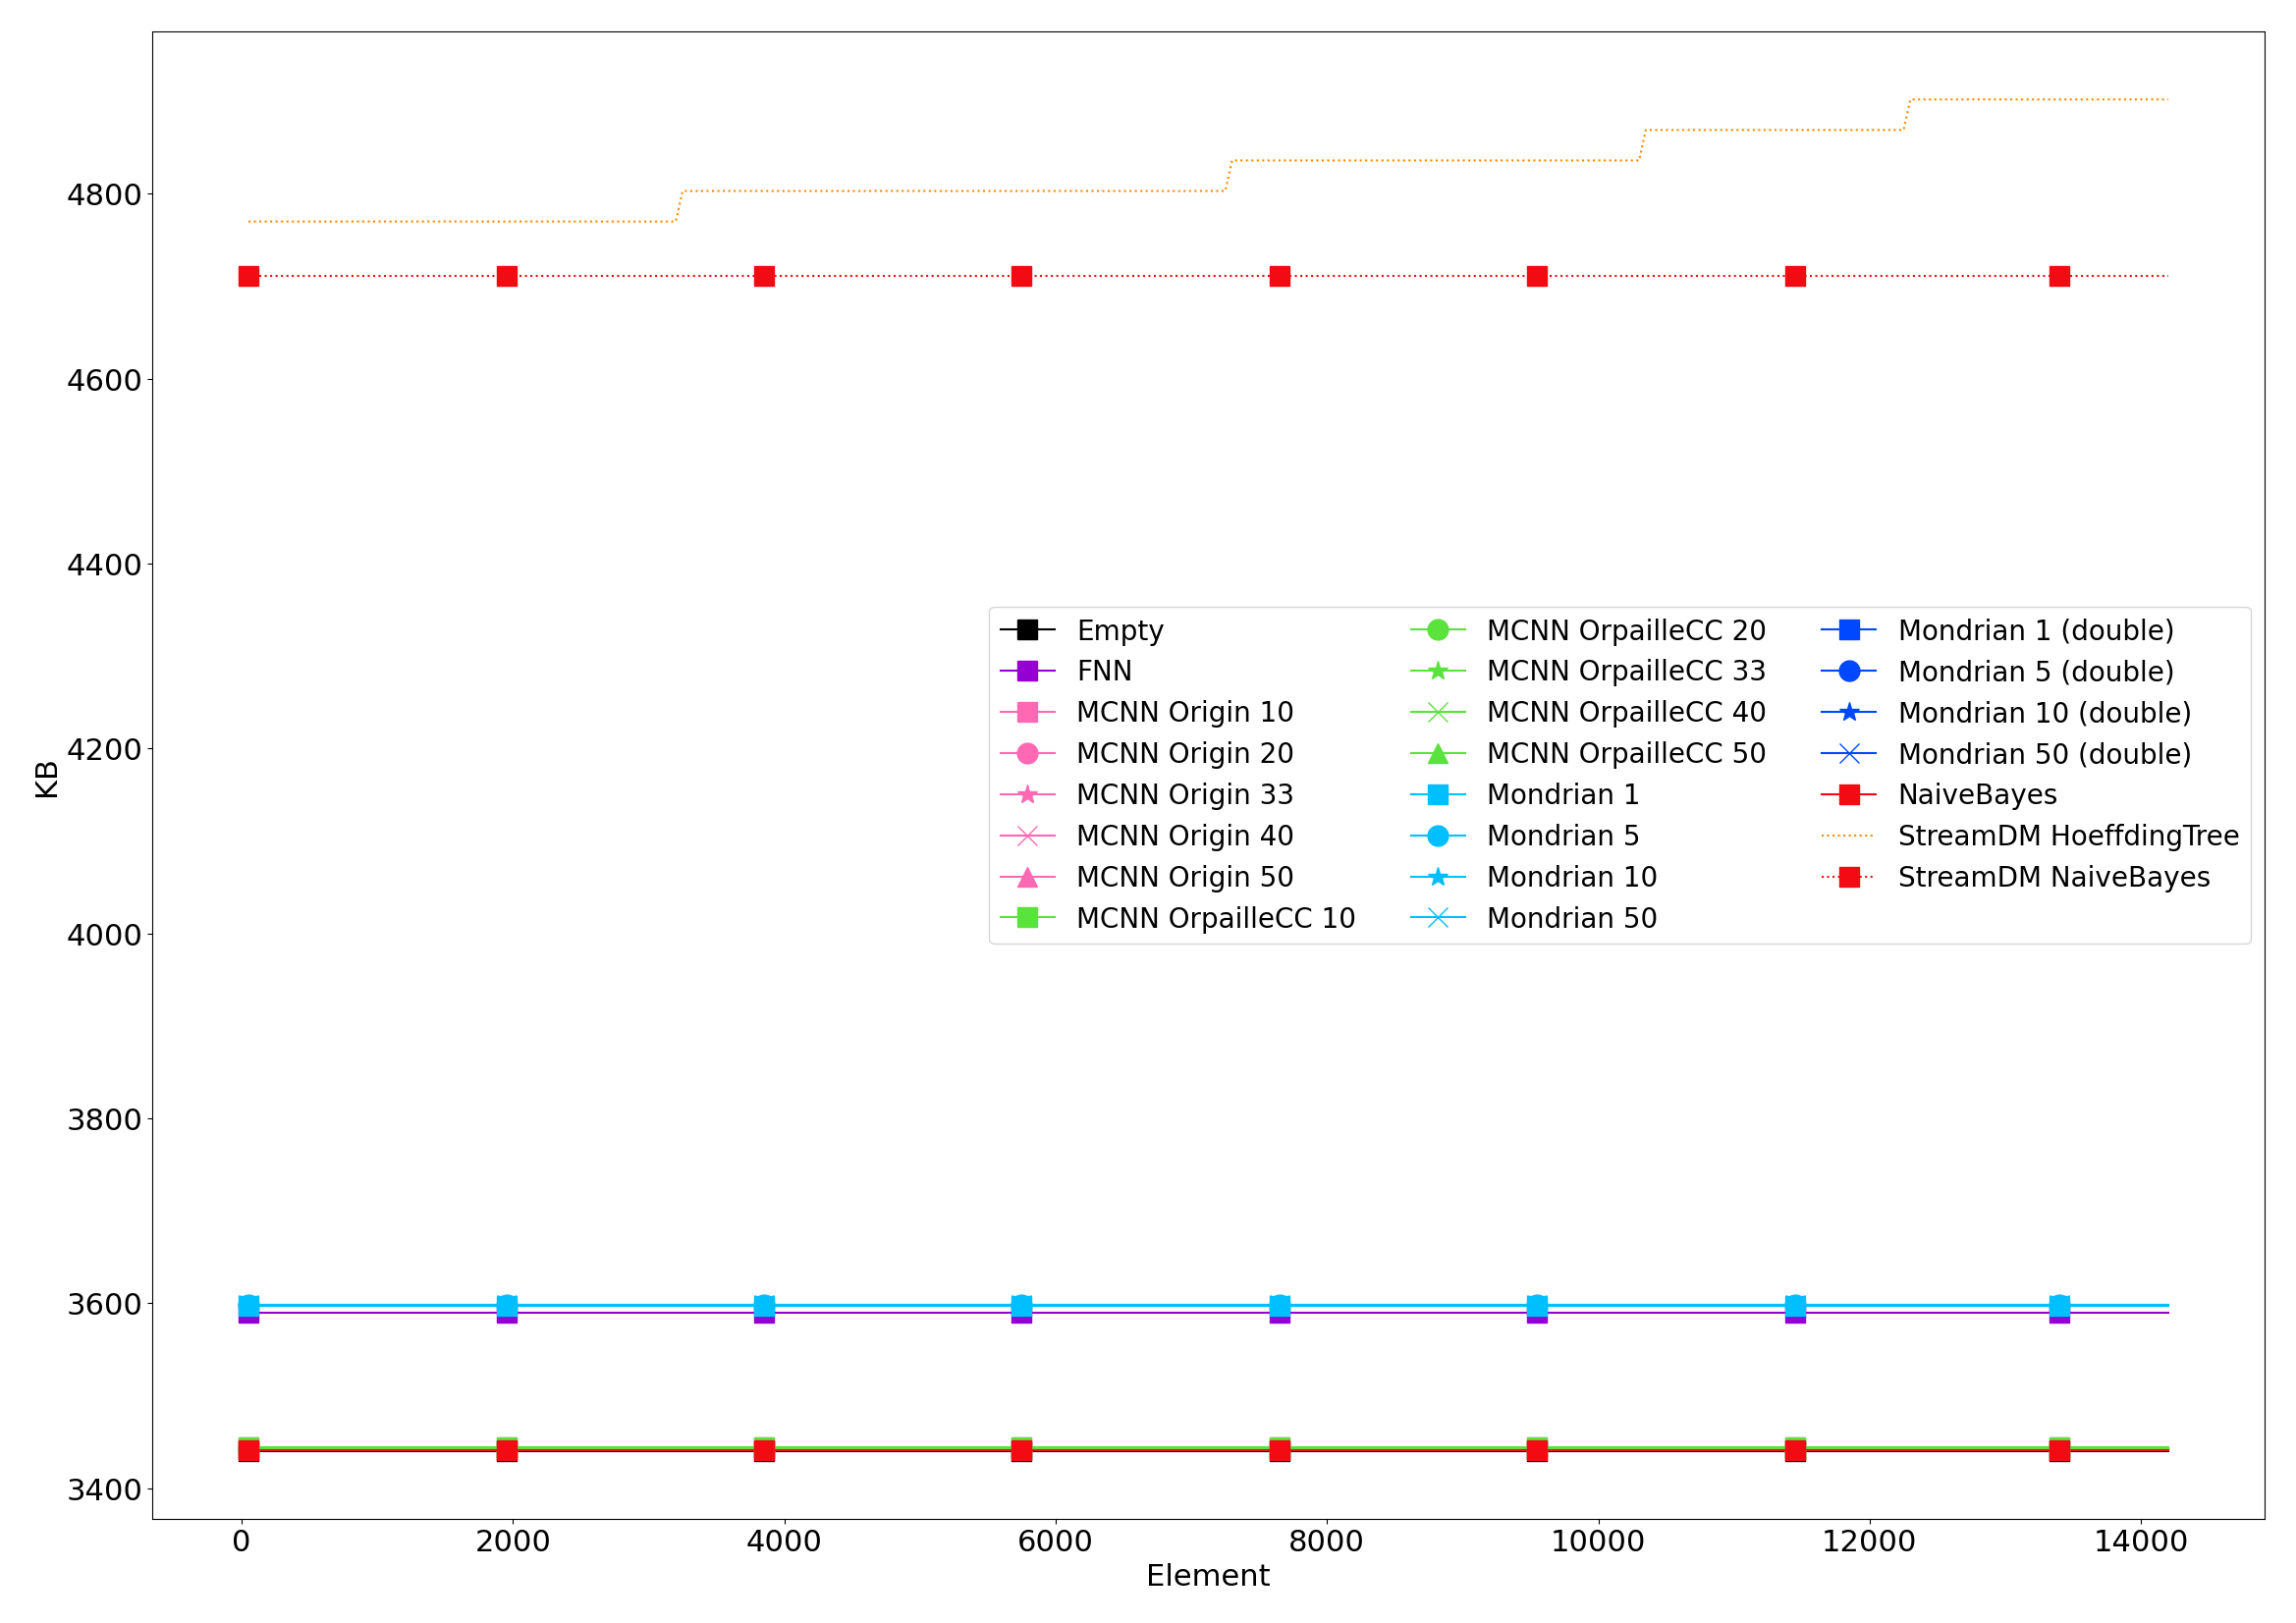
\includegraphics[width=\linewidth]{figures/results/banos_3_memory.png}
	\caption{Memory used by the algorithms on the Banos dataset. \TG{increase font size in all graphs, to make it only slightly smaller than font size in caption}}
	\label{fig:memory}
\end{figure}


\subsection{Micro-Cluster Nearest Neighbor Hyperparameters}

Figure~\ref{fig:mcnn-tuning-error} shows the impact of the error threshold
in the MCNN classifiers. The higher the number of clusters, the better are
the performance \TG{ok but the number of clusters isn't a hyper parameter,
this should be moved to the description of F1 score results}. The error
threshold of MCNN has little impact on the classification performance. For
20 and 40 clusters, the best-performing threshold is either 2 or 4, meaning
that a cluster may do 2 or 4 errors before being split. For 10 clusters,
all error thresholds perform equally.

\begin{figure}
	 \begin{subfigure}[b]{0.49\textwidth}
		 \centering
		 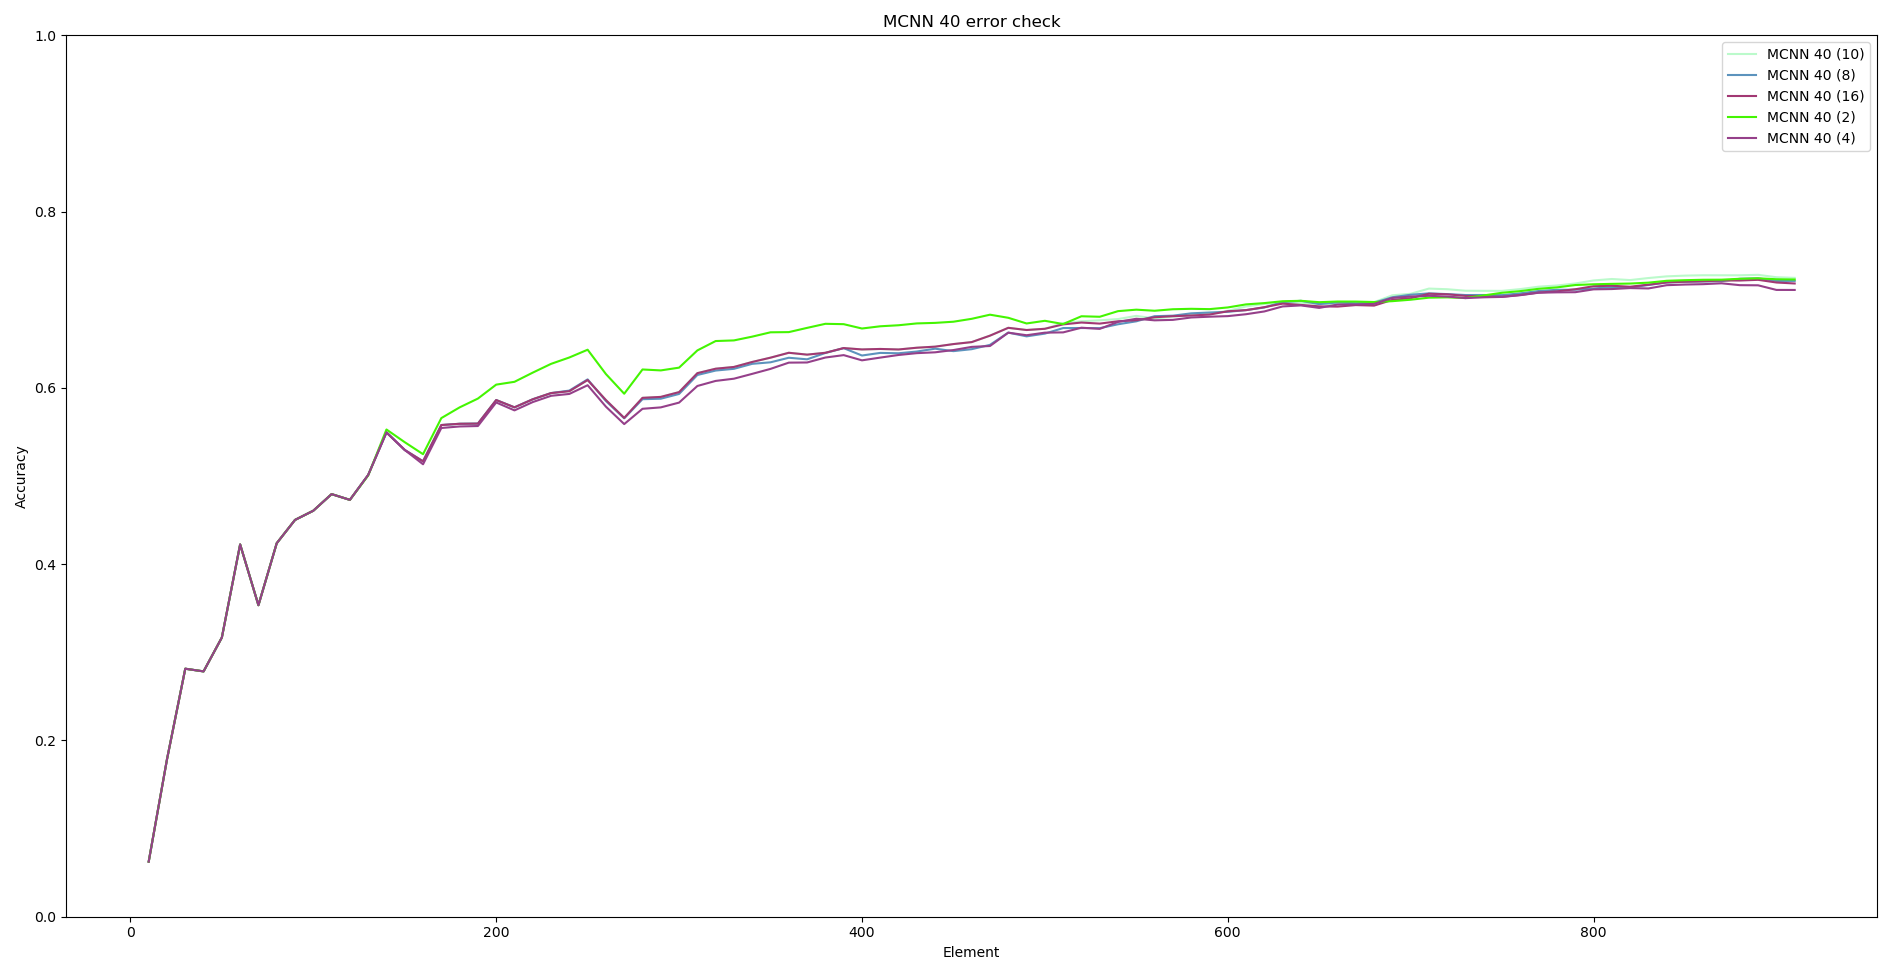
\includegraphics[width=\linewidth]{figures/Banos_S1_shuf_MCNN_40_error_check.png}
		 \caption{40 clusters}
	 \end{subfigure}
	 \begin{subfigure}[b]{0.49\textwidth}
		 \centering
		 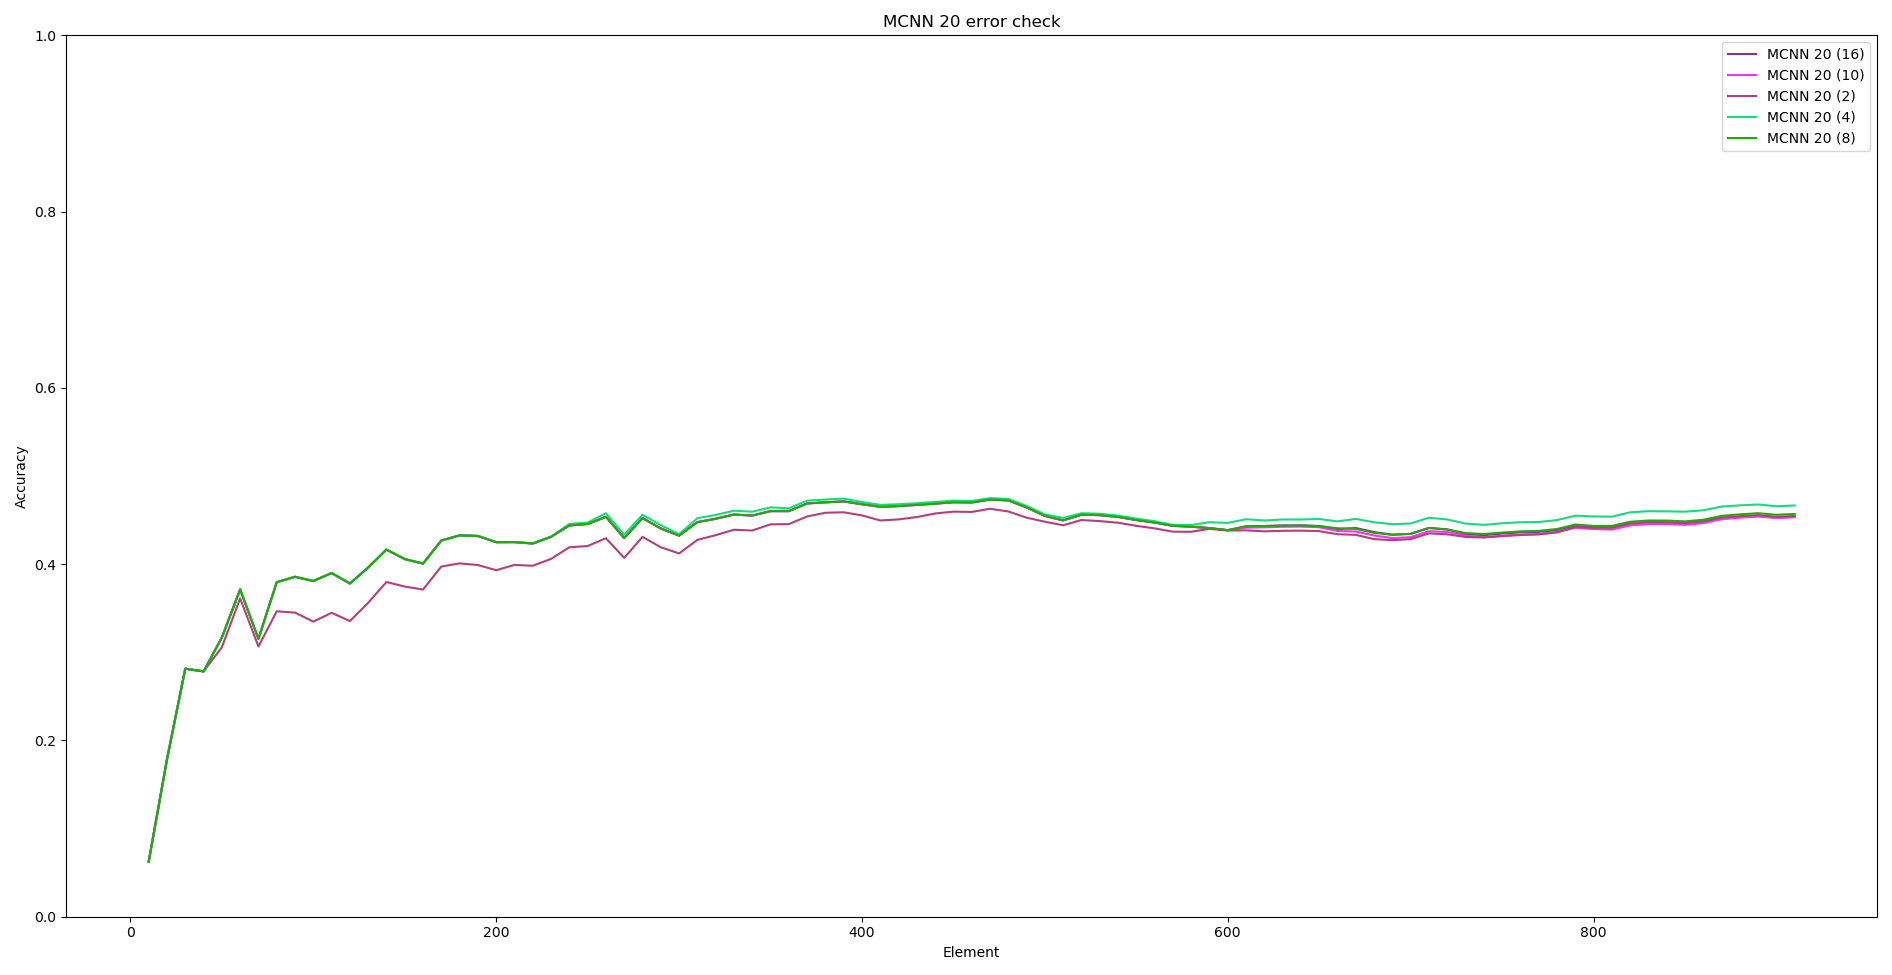
\includegraphics[width=\linewidth]{figures/Banos_S1_shuf_MCNN_20_error_check.png}
		 \caption{20 clusters}
	 \end{subfigure}
	 \begin{subfigure}[b]{0.49\textwidth}
		 \centering
		 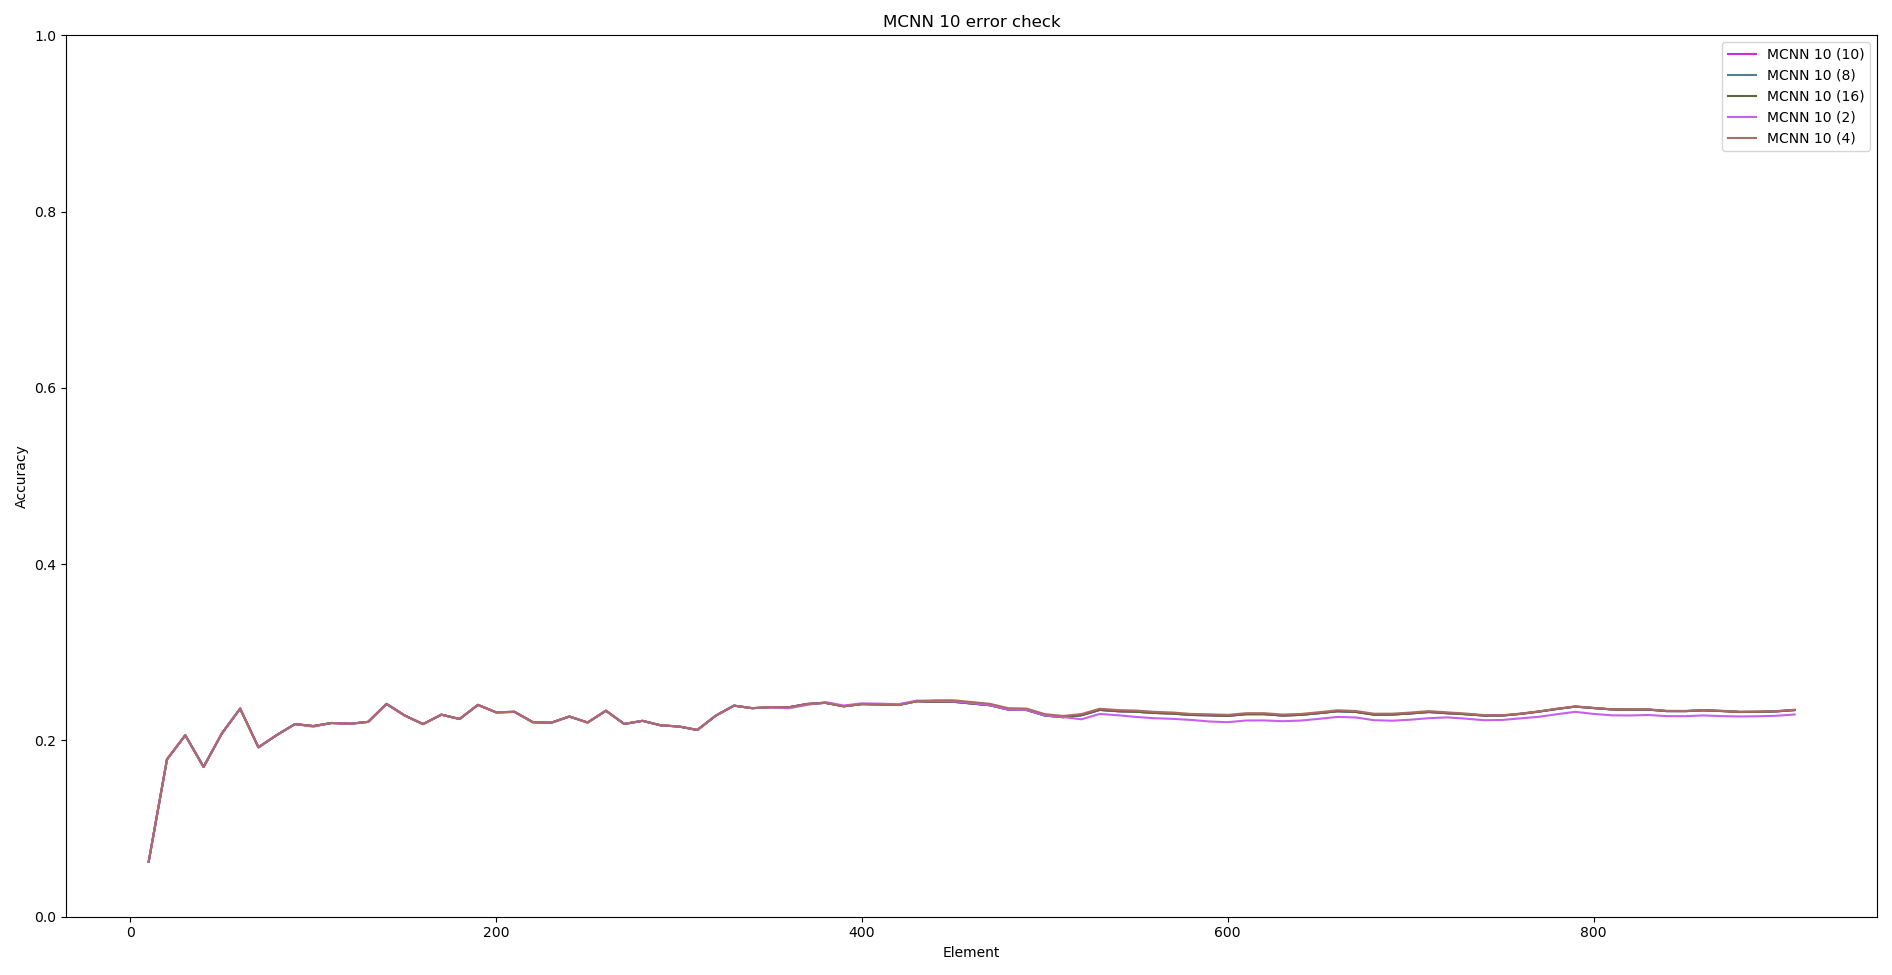
\includegraphics[width=\linewidth]{figures/Banos_S1_shuf_MCNN_10_error_check.png}
		 \caption{10 clusters}
	 \end{subfigure}
	\caption{Impact of the error threshold on MCNN performance (first subject of \banosdataset dataset). \TG{It's a bit weird to use accuracy here while F1 score was used before. 
	Couldn't you just use F1 score here too?}}
	\label{fig:mcnn-tuning-error}
\end{figure}

\subsection{Mondrian Forest Hyperparameters}

Figure~\ref{fig:mondrian-tuning} shows the impact of the Mondrian Forest hyperparameters on
the classification performance. Occasionally, dashed lines are used to
emphasize the minimum and the maximum \TG{That's a comment for the caption. Why ``occasionally'' and not always?}.

The base count hyperparameter (Figure~\ref{fig:mondrian-base-count}) has a
very substantial impact on classification performance; the smallest value
(\TG{add value here}) results in the best performance. On the contrary, the
budget hyperparameter (Figure~\ref{fig:mondrian-budget}) only has a
moderate impact on classification; the best value is slightly below
1.0. Finally, the discount hyperparameter
(Figure~\ref{fig:mondrian-discount}) has a negligible impact on the
performance; the best-performing value is 0.1.

\TG{Add the selected values of hyperparameters somewhere before, maybe in sub-figure captions in F1 scores.}

\begin{figure}
	 \centering
	 \begin{subfigure}[b]{0.49\textwidth}
		\centering
		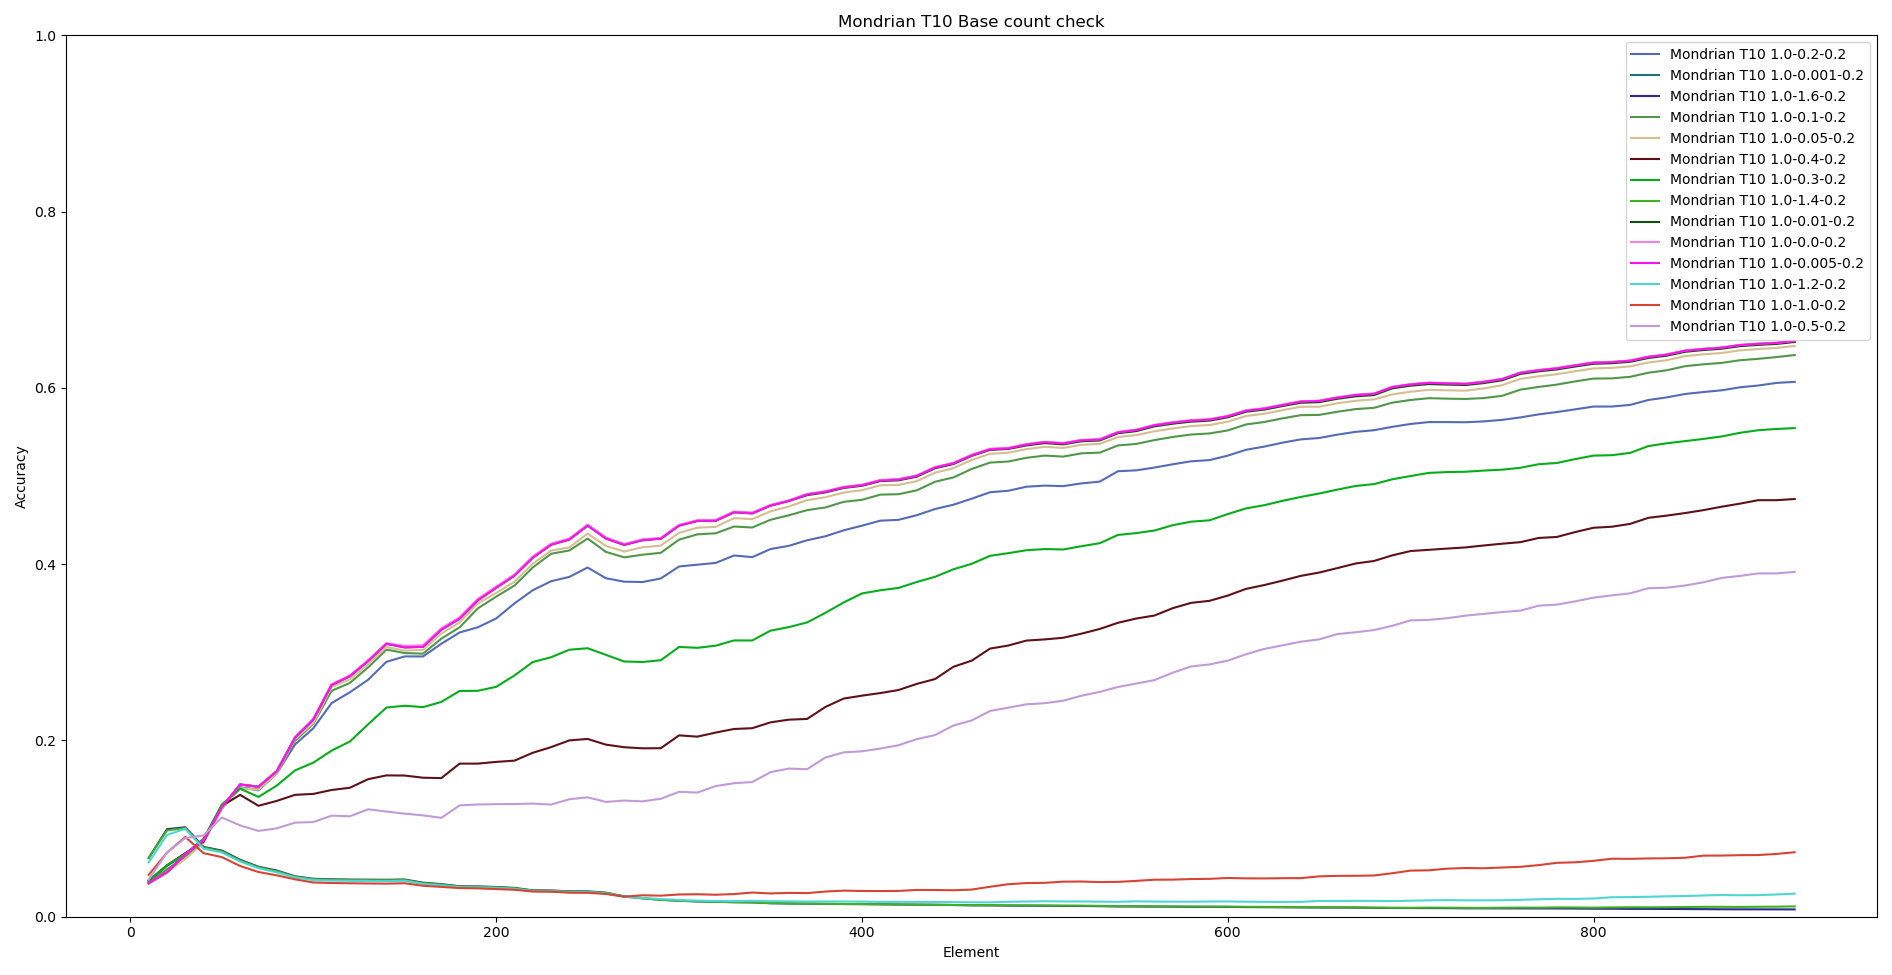
\includegraphics[width=\textwidth]{figures/Banos_S1_shuf_Mondrian_T10_check.png}
		\caption{Impact of the base count with 10 trees, a budget of $1.0$, and a discount factor of $0.2$. \TG{Could you simplify the figure legend to just show ``Mondrian - <base count>''? 
		it's a bit difficult to read and all parameters are the same and reported in this caption. Same comment for the other sub-figures.}} 
		\label{fig:mondrian-base-count}
	\end{subfigure}
	\hfill
	 \begin{subfigure}[b]{0.49\textwidth}
		 \centering
		 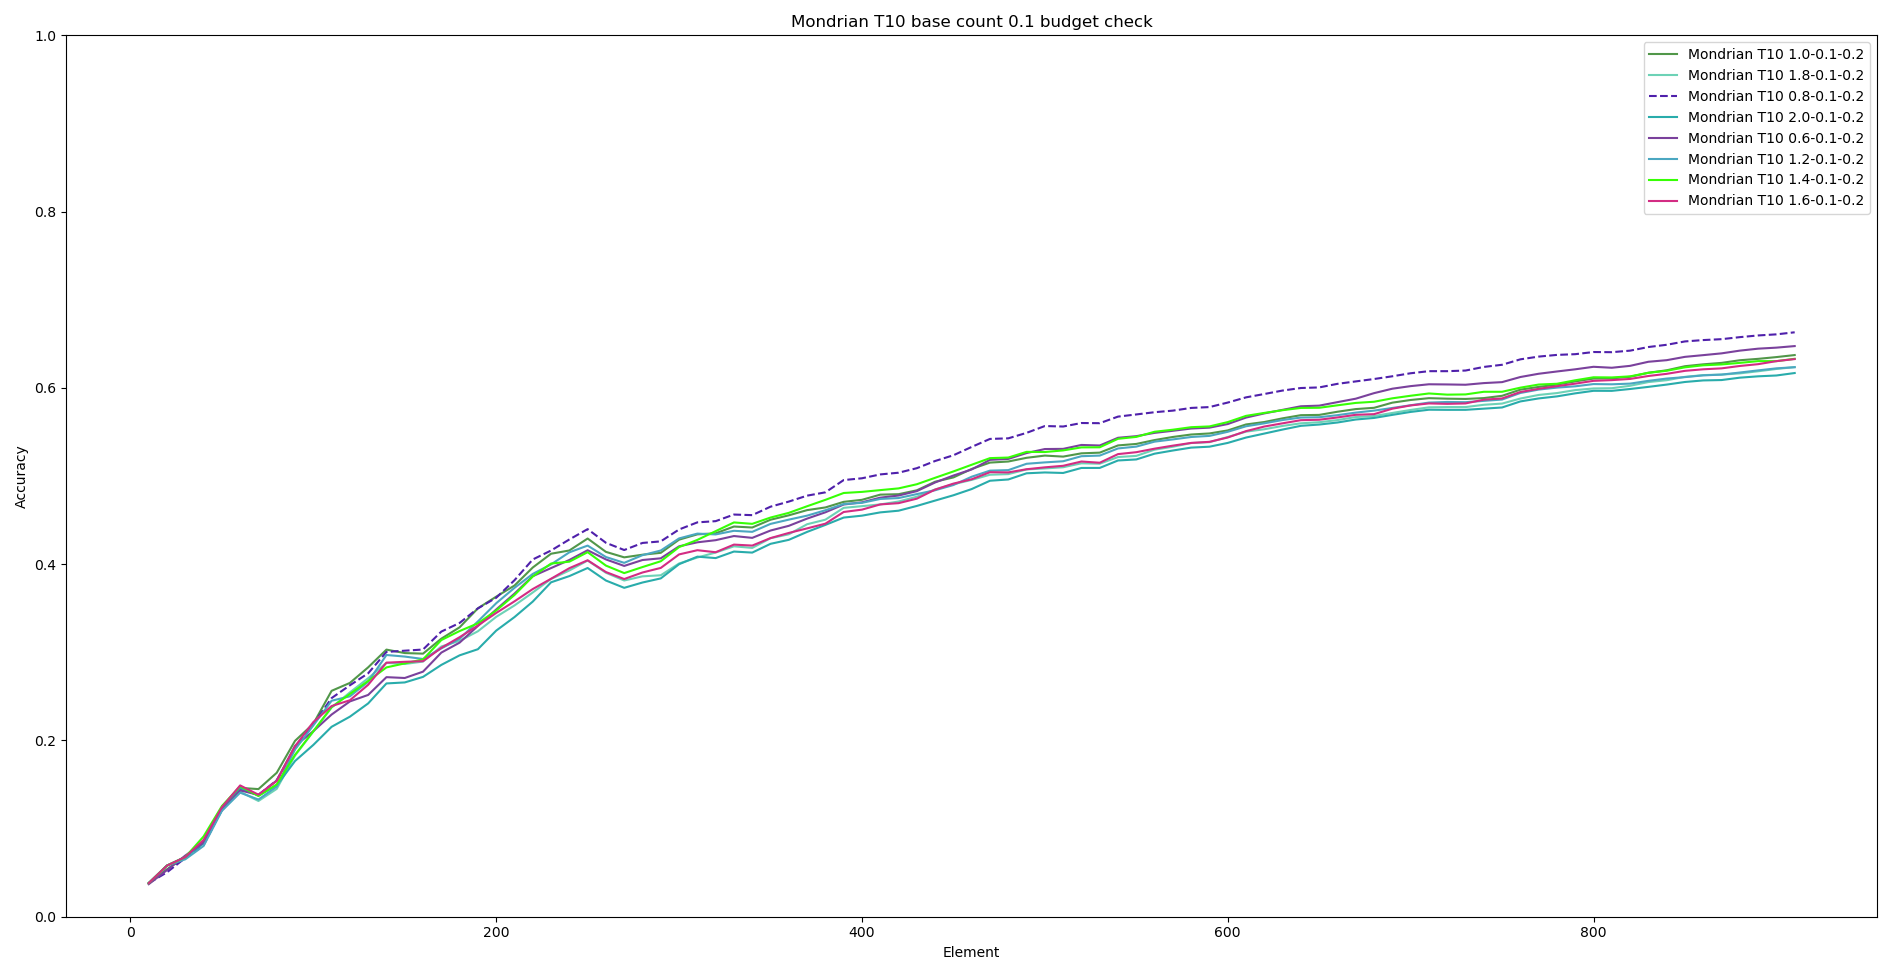
\includegraphics[width=\textwidth]{figures/Banos_S1_shuf_Mondrian_T10_bc_0.1_budget_check.png}
		 \caption{Impact of the budget with 10 trees, a base count of $0.1$, and discount factor of $0.2$.}
		 \label{fig:mondrian-budget}
	 \end{subfigure}
	 \hfill
	 \begin{subfigure}[b]{0.49\textwidth}
		 \centering
		 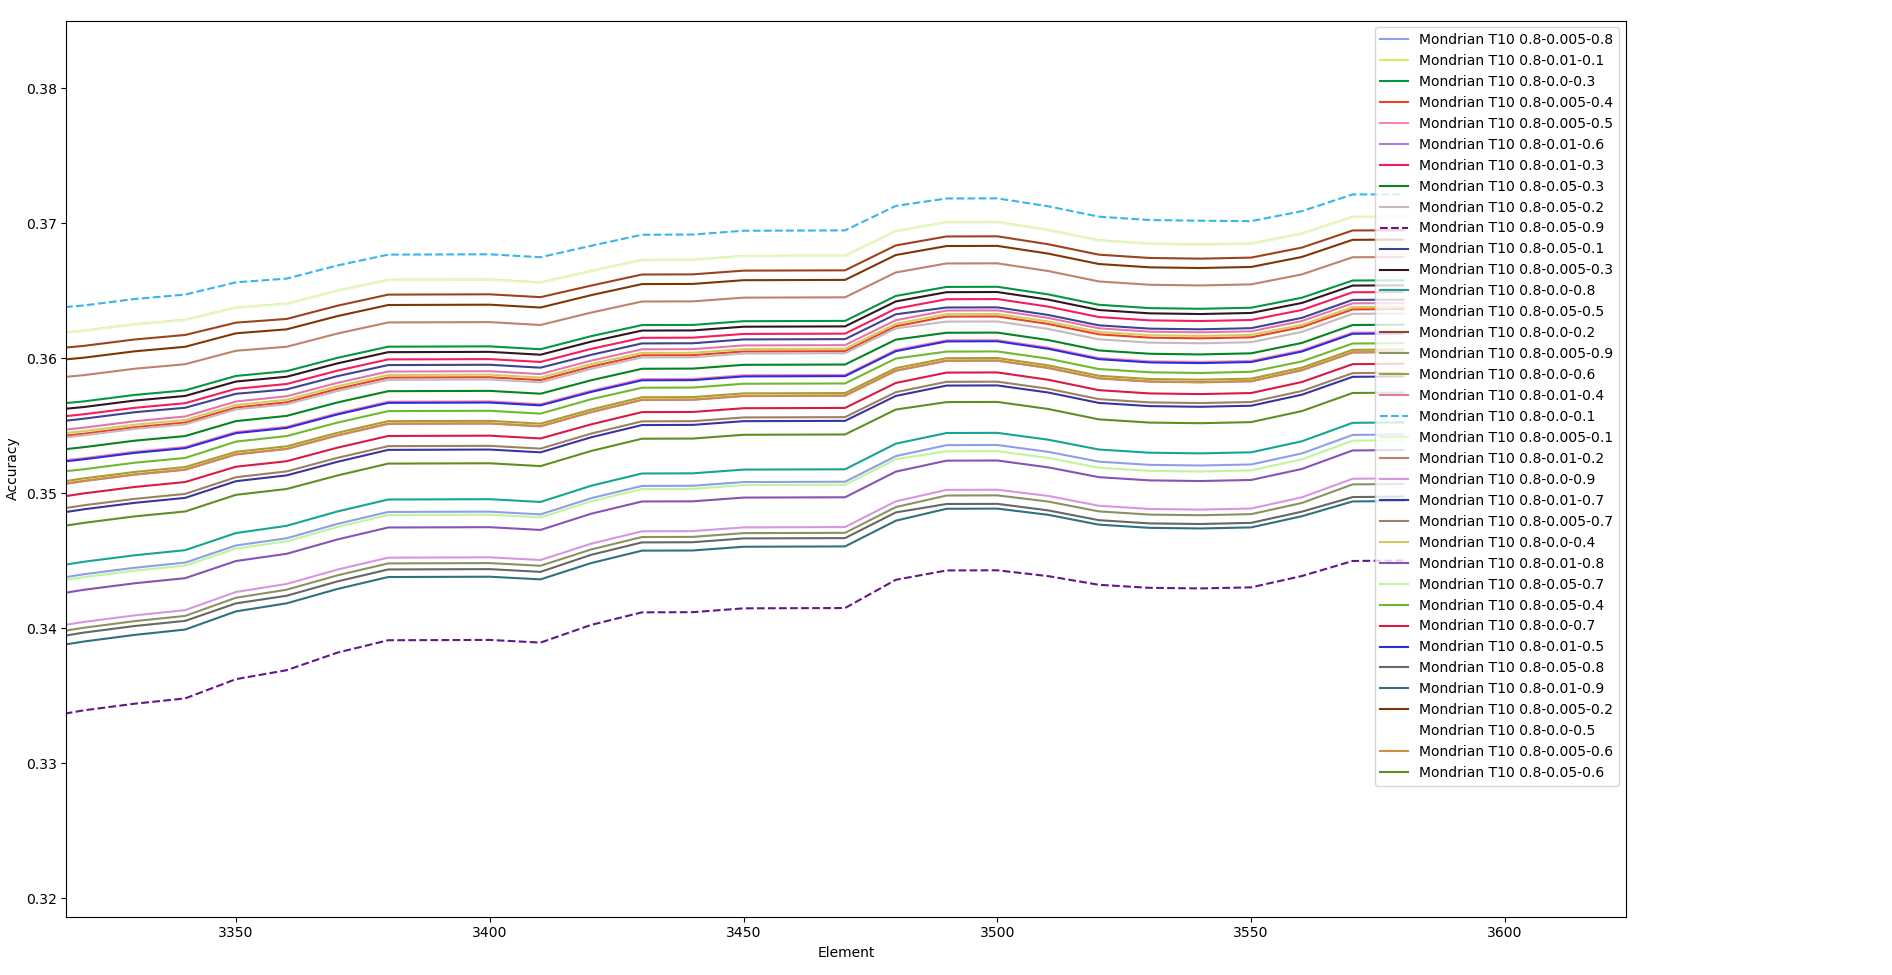
\includegraphics[width=\textwidth]{figures/Banos_S1_disount_check.png}
		 \caption{Impact of the discount factor with 10 trees, a budget of $1.0$, and a base count of $0.1$. \TG{put this graph on the same 0-1 scale as the two other ones.}}
		 \label{fig:mondrian-discount}
	 \end{subfigure}
		\caption{Mondrian tuning results.}
		\label{fig:mondrian-tuning}
\end{figure}


